\chapter{士師記}

\section{序言 1:1-3:6 }
\subsection{繼續攻打迦南地 1:1-26 }

\begin{figure}[!htb]  
	 \begin{center}
	 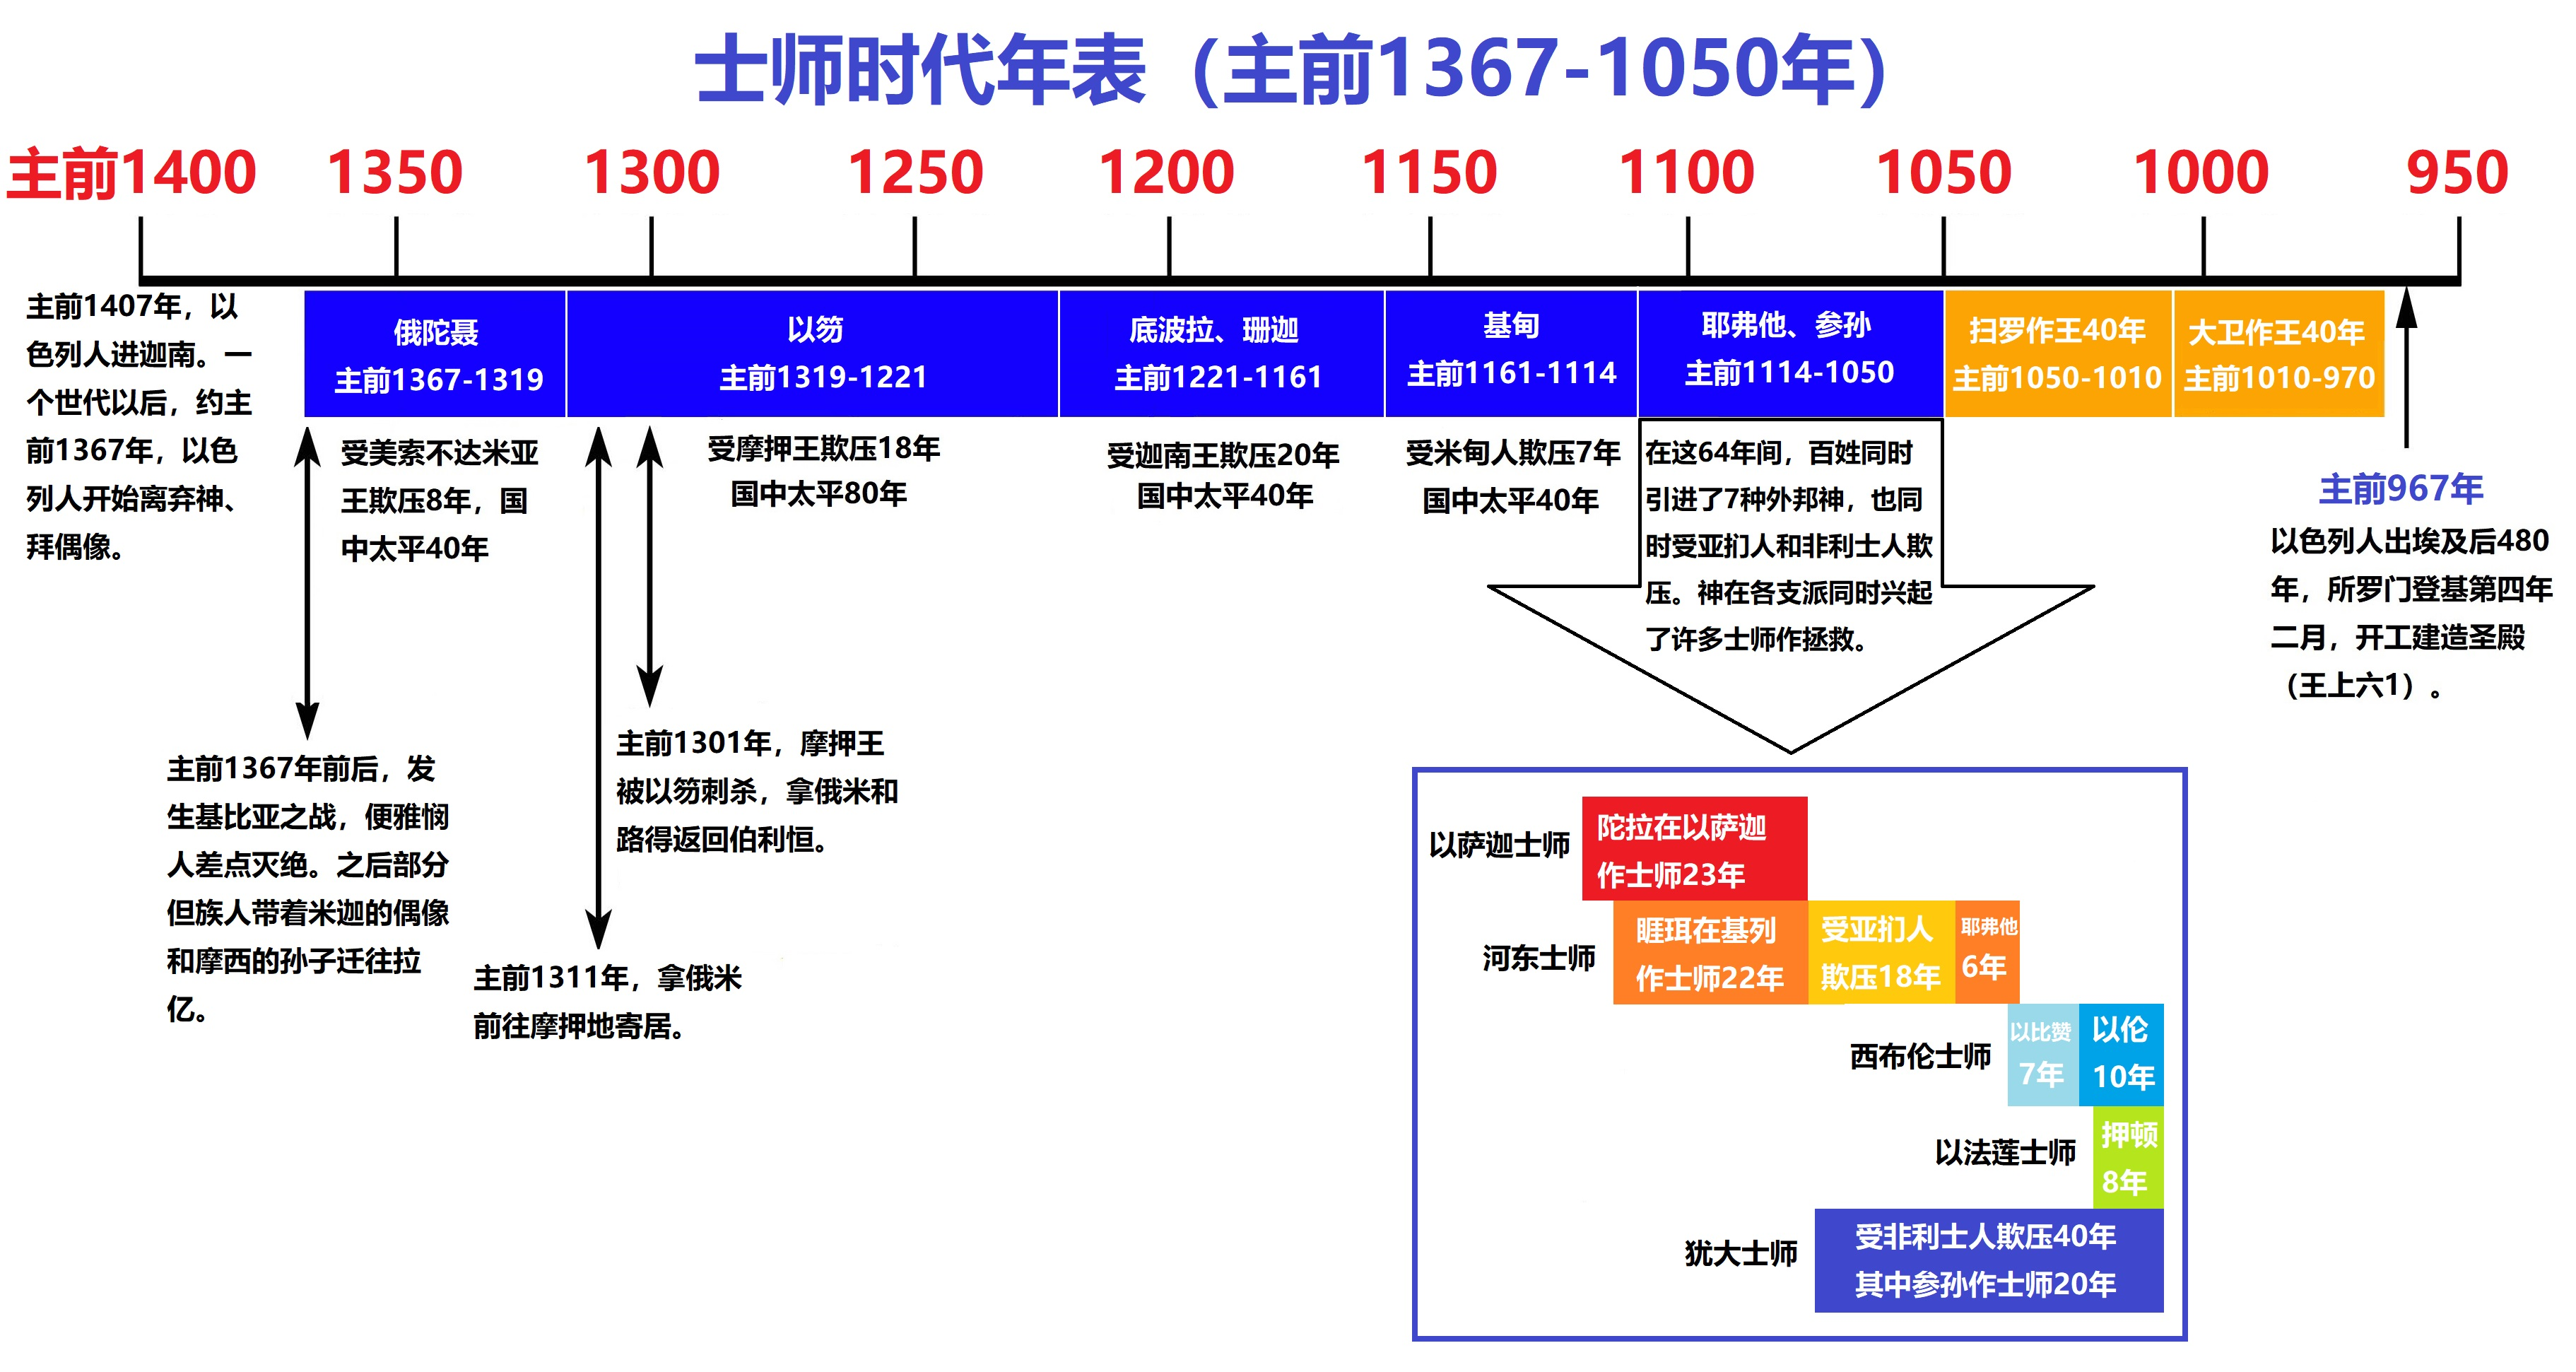
\includegraphics[width=7in]{BLiShiFigs/judge/judges}
	 \caption{士師時期}
%	 \label{fig:1} 
	 \end{center}
	 \end{figure}

\begin{table}[H]
\centering
\begin{tabular}{|c|c|c|c|}
\hline
\hline
支派                 &地點 & 敵人                     & 殺的人    \\\hline\hline
猶大,西緬     & 比色  & 迦南人和比利洗人    & 亞多尼比色      \\\hline
猶大     & 耶路撒冷  &               &       \\\hline
猶大     &  山地、南地和高原       &迦南人                    &         \\\hline
猶大    &希伯崙(基列亞巴) &迦南人 &   示篩、亞希幔、撻買\\\hline
猶大 &底壁(基列西弗，俄陀聶娶押撒） &  & \\\hline
猶大,西緬&何珥瑪(洗法)& 迦南人  & \\\hline
猶大& 迦薩，亞實基倫，以革倫&   &  \\\hline
迦勒& 希伯崙&亞衲族的三個族長& \\\hline
約瑟&伯特利（路斯）  & & \\\hline
\end{tabular}
\caption{以色列人攻打的地方}
\end{table}

\subsubsection{猶大西緬在比色殺敗迦南人和比利洗人 1:1-7}
約書亞死後，以色列人求問耶和華說：「我們中間誰當首先上去攻擊迦南人，與他們爭戰？」 2 耶和華說：「猶大當先上去，我已將那地交在他手中。」 3 猶大對他哥哥西緬說：「請你同我到拈鬮所得之地去，好與迦南人爭戰，以後我也同你到你拈鬮所得之地去。」於是西緬與他同去。 4 猶大就上去，耶和華將迦南人和比利洗人交在他們手中，他們在比色擊殺了一萬人。 5 又在那裡遇見亞多尼比色，與他爭戰，殺敗迦南人和比利洗人。 6 亞多尼比色逃跑，他們追趕，拿住他，砍斷他手腳的大拇指。 7 亞多尼比色說：「從前有七十個王，手腳的大拇指都被我砍斷，在我桌子底下拾取零碎食物。現在神按著我所行的報應我了。」於是他們將亞多尼比色帶到耶路撒冷，他就死在那裡。

\subsubsection{猶大攻打耶路撒冷希伯崙 1:8-10}
猶大人攻打耶路撒冷，將城攻取，用刀殺了城內的人，並且放火燒城。 9 後來猶大人下去，與住山地、南地和高原的迦南人爭戰。 10 猶大人去攻擊住希伯崙的迦南人，殺了示篩、亞希幔、撻買，希伯崙從前名叫基列亞巴。

\subsubsection{猶大攻打底璧(基列西弗) 1:11-15}
他們從那裡去攻擊底璧的居民，底璧從前名叫基列西弗。 12 迦勒說：「誰能攻打基列西弗，將城奪取，我就把我女兒押撒給他為妻。」 13 迦勒兄弟基納斯的兒子俄陀聶奪取了那城，迦勒就把女兒押撒給他為妻。 14 押撒過門的時候，勸丈夫向她父親求一塊田。押撒一下驢，迦勒問她說：「你要什麼？」 15 她說：「求你賜福給我，你既將我安置在南地，求你也給我水泉。」迦勒就把上泉下泉賜給她。

\subsubsection{摩西的內兄基尼人住在猶大曠野 1:16}
摩西的內兄(岳父)是基尼人，他的子孫與猶大人一同離了棕樹城，往亞拉得以南的猶大曠野去，就住在民中。

\subsubsection{猶大西緬取了洗法 1:16}
猶大和他哥哥西緬同去，擊殺了住洗法的迦南人，將城盡行毀滅，那城的名便叫何珥瑪。

\subsubsection{猶大攻取了加沙和四境 1:17-20}
猶大又取了加沙和加沙的四境，亞實基倫和亞實基倫的四境，以革倫和以革倫的四境。耶和華與猶大同在，猶大就趕出山地的居民，只是不能趕出平原的居民，因為他們有鐵車。以色列人照摩西所說的，將希伯崙給了迦勒，迦勒就從那裡趕出亞衲族的三個族長。

\subsubsection{便雅憫人沒有趕出耶布斯人 1:21}
便雅憫人沒有趕出住耶路撒冷的耶布斯人，耶布斯人仍在耶路撒冷與便雅憫人同住，直到今日。

\subsubsection{約瑟家攻打伯特利 1:22-26}
約瑟家也上去攻打伯特利，耶和華與他們同在。 23 約瑟家打發人去窺探伯特利，那城起先名叫路斯。 24 窺探的人看見一個人從城裡出來，就對他說：「求你將進城的路指示我們，我們必恩待你。」 25 那人將進城的路指示他們，他們就用刀擊殺了城中的居民，但將那人和他全家放去。 26 那人往赫人之地去，築了一座城，起名叫路斯，那城到如今還叫這名。

\subsection{以色列人的失败 1:27-3:6}
\subsubsection{以色列人未得之地 1:27-36}
\begin{table}[!hbp]
\centering
\begin{tabular}{|c|c|c|c|}
\hline
\hline
支派                 &未得之地地點 & 敵人     &    原因               \\\hline\hline
猶大     & 平原的居民  &      &       有鐵車  \\\hline
便雅憫     & 耶路撒冷  &     耶布斯人          &       \\\hline
瑪拿西    &伯善,他納，多珥,以伯蓮,米吉多 &迦南  &    \\\hline
以法蓮 &基色 & 迦南人 & \\\hline
西布倫&基倫,拿哈拉& 迦南人  & \\\hline
亞設& 亞柯,西頓，亞黑拉,亞革悉，黑巴、亞弗革,利合&   &  \\\hline
拿弗他利& 伯示麥,伯亞納&亞衲族的三個族長& \\\hline
但&平原  &亞摩利 & \\\hline
\end{tabular}
\caption{以色列人未得之地}
\end{table}

\begin{table}[H]
\centering
\begin{tabular}{p{4.4cm}|p{1.45cm}|p{1.8cm}|p{2.55cm}|p{2.3cm}|p{3.25cm}}\hline\hline
瑪拿西&以法蓮&西布倫&亞設&拿弗他利&但\\\hline
瑪拿西沒有趕出伯善和屬伯善鄉村的居民，他納和屬他納鄉村的居民，多珥和屬多珥鄉村的居民，以伯蓮和屬以伯蓮鄉村的居民，米吉多和屬米吉多鄉村的居民，迦南人卻執意住在那些地方。及至以色列強盛了就使迦南人做苦工沒有把他們全然趕出
&以法蓮沒有趕出住基色的迦南人，於是迦南人仍住在基色在以法蓮中間。
&西布倫沒有趕出基倫的居民和拿哈拉的居民於是迦南人仍住在西布倫中間成了服苦的人
&亞設沒有趕出亞柯和西頓的居民,亞黑拉和亞革悉的居民,黑巴、亞弗革與利合的居民。於是亞設因為沒有趕出那地的迦南人就住在他們中間
&拿弗他利沒有趕出伯示麥和伯亞納的居民，於是拿弗他利就住在那地的迦南人中間，然而伯示麥和伯亞納的居民成了服苦的人。
&亞摩利人強逼但人住在山地不容他們下到平原。亞摩利人卻執意住在希烈山和亞雅倫並沙賓，然而約瑟家勝了他們使他們成了服苦的人。亞摩利人的境界是從亞克拉濱坡從西拉而上\\\hline
 \end{tabular}
\caption{以色列人未得之地}
\end{table}

 
\subsubsection{耶和華的使者在波金責備以色列人 2:1-5}
耶和華的使者從吉甲上到波金，對以色列人說：「我使你們從埃及上來，領你們到我向你們列祖起誓應許之地。我又說：『我永不廢棄與你們所立的約， 2 你們也不可與這地的居民立約，要拆毀他們的祭壇。』你們竟沒有聽從我的話。為何這樣行呢？ 3 因此我又說：我必不將他們從你們面前趕出，他們必做你們肋下的荊棘，他們的神必做你們的網羅。」 4 耶和華的使者向以色列眾人說這話的時候，百姓就放聲而哭。 5 於是給那地方起名叫波金 a。眾人在那裡向耶和華獻祭。

\subsubsection{約書亞辭世 2:6-10 }
從前約書亞打發以色列百姓去的時候，他們各歸自己的地業，占據地土。 7 約書亞在世和約書亞死後，那些見耶和華為以色列人所行大事的長老還在的時候，百姓都侍奉耶和華。 8 耶和華的僕人嫩的兒子約書亞，正一百一十歲就死了。 9 以色列人將他葬在他地業的境內，就是在以法蓮山地的亭拿希烈，在迦實山的北邊。 10 那世代的人也都歸了自己的列祖。後來有別的世代興起，不知道耶和華，也不知道耶和華為以色列人所行的事。

\subsubsection{以色列人惡性循環 2:11-23 }
\begin{table}[H]
\centering
\begin{tabular}{p{2.7cm}|p{3.7cm}|p{4.5cm}|p{5.6cm}}\hline\hline
離棄耶和華&被交給仇敵&上帝興起士師拯救&不再趕出各族\\\hline
以色列人行耶和華眼中看為惡的事，去侍奉諸巴力，離棄了領他們出埃及地的耶和華他們列祖的神，去叩拜別神，就是四圍列國的神，惹耶和華發怒；並離棄耶和華，去侍奉巴力和亞斯她錄。
&耶和華的怒氣向以色列人發作，就把他們交在搶奪他們的人手中，又將他們付於四圍仇敵的手中，甚至他們在仇敵面前再不能站立得住。他們無論往何處去，耶和華都以災禍攻擊他們，正如耶和華所說的話，又如耶和華向他們所起的誓。他們便極其困苦。
&耶和華興起士師，士師就拯救他們脫離搶奪他們人的手。他們卻不聽從士師，竟隨從叩拜別神行了邪淫，速速地偏離他們列祖所行的道，不如他們列祖順從耶和華的命令。耶和華為他們興起士師，就與那士師同在，士師在世的一切日子，耶和華拯救他們脫離仇敵的手；他們因受欺壓擾害就哀聲嘆氣，所以耶和華後悔了。
&及至士師死後，他們就轉去行惡，比他們列祖更甚，去侍奉叩拜別神，總不斷絕頑梗的惡行。於是耶和華的怒氣向以色列人發作，他說：「因這民違背我吩咐他們列祖所守的約，不聽從我的話，所以約書亞死的時候所剩下的各族，我必不再從他們面前趕出，為要藉此試驗以色列人，看他們肯照他們列祖謹守遵行我的道不肯。」這樣，耶和華留下各族，不將他們速速趕出，也沒有交付約書亞的手。\\\hline
 \end{tabular}
\caption{以色列人未得之地}
\end{table}

\hspace*{30mm}
\smartdiagram[flow diagram:horizontal]{以色列人犯罪,
  被交給仇敵, 百姓呼求神, 上帝興起士師拯救, 平安一段時期直到士師死}

\subsubsection{存留的迦南各族人 3:1-6}
\begin{wraptable}{r}{8cm}
\vspace*{-10mm}
\centering
\begin{tabular}{|c|c|}\hline
存留的迦南各族人                &居住地   \\\hline\hline
非利士五首領 &    \\\hline
西頓人    &  \\\hline
希未人   &  利巴嫩山(巴力黑們山->哈馬口)\\\hline
迦南人&  \\\hline
赫人  & \\\hline
亞摩利人&  \\\hline
比利洗人 &  \\\hline
耶布斯人 & \\\hline
\end{tabular}
\caption{存留的迦南各族人}
\end{wraptable}
耶和華留下這幾族，為要試驗那不曾知道與迦南爭戰之事的以色列人，好叫以色列的後代又知道又學習未曾曉得的戰事。所留下的就是非利士的五個首領和一切迦南人，西頓人，並住黎巴嫩山的希未人（從巴力黑們山直到哈馬口）。留下這幾族，為要試驗以色列人，知道他們肯聽從耶和華藉摩西吩咐他們列祖的誡命不肯。以色列人竟住在迦南人、赫人、亞摩利人、比利洗人、希未人、耶布斯人中間，娶他們的女兒為妻，將自己的女兒嫁給他們的兒子，並侍奉他們的神。


\section{士師时期 3:7-16:31}
    \begin{figure}[!htb]  
	 \begin{center}
	 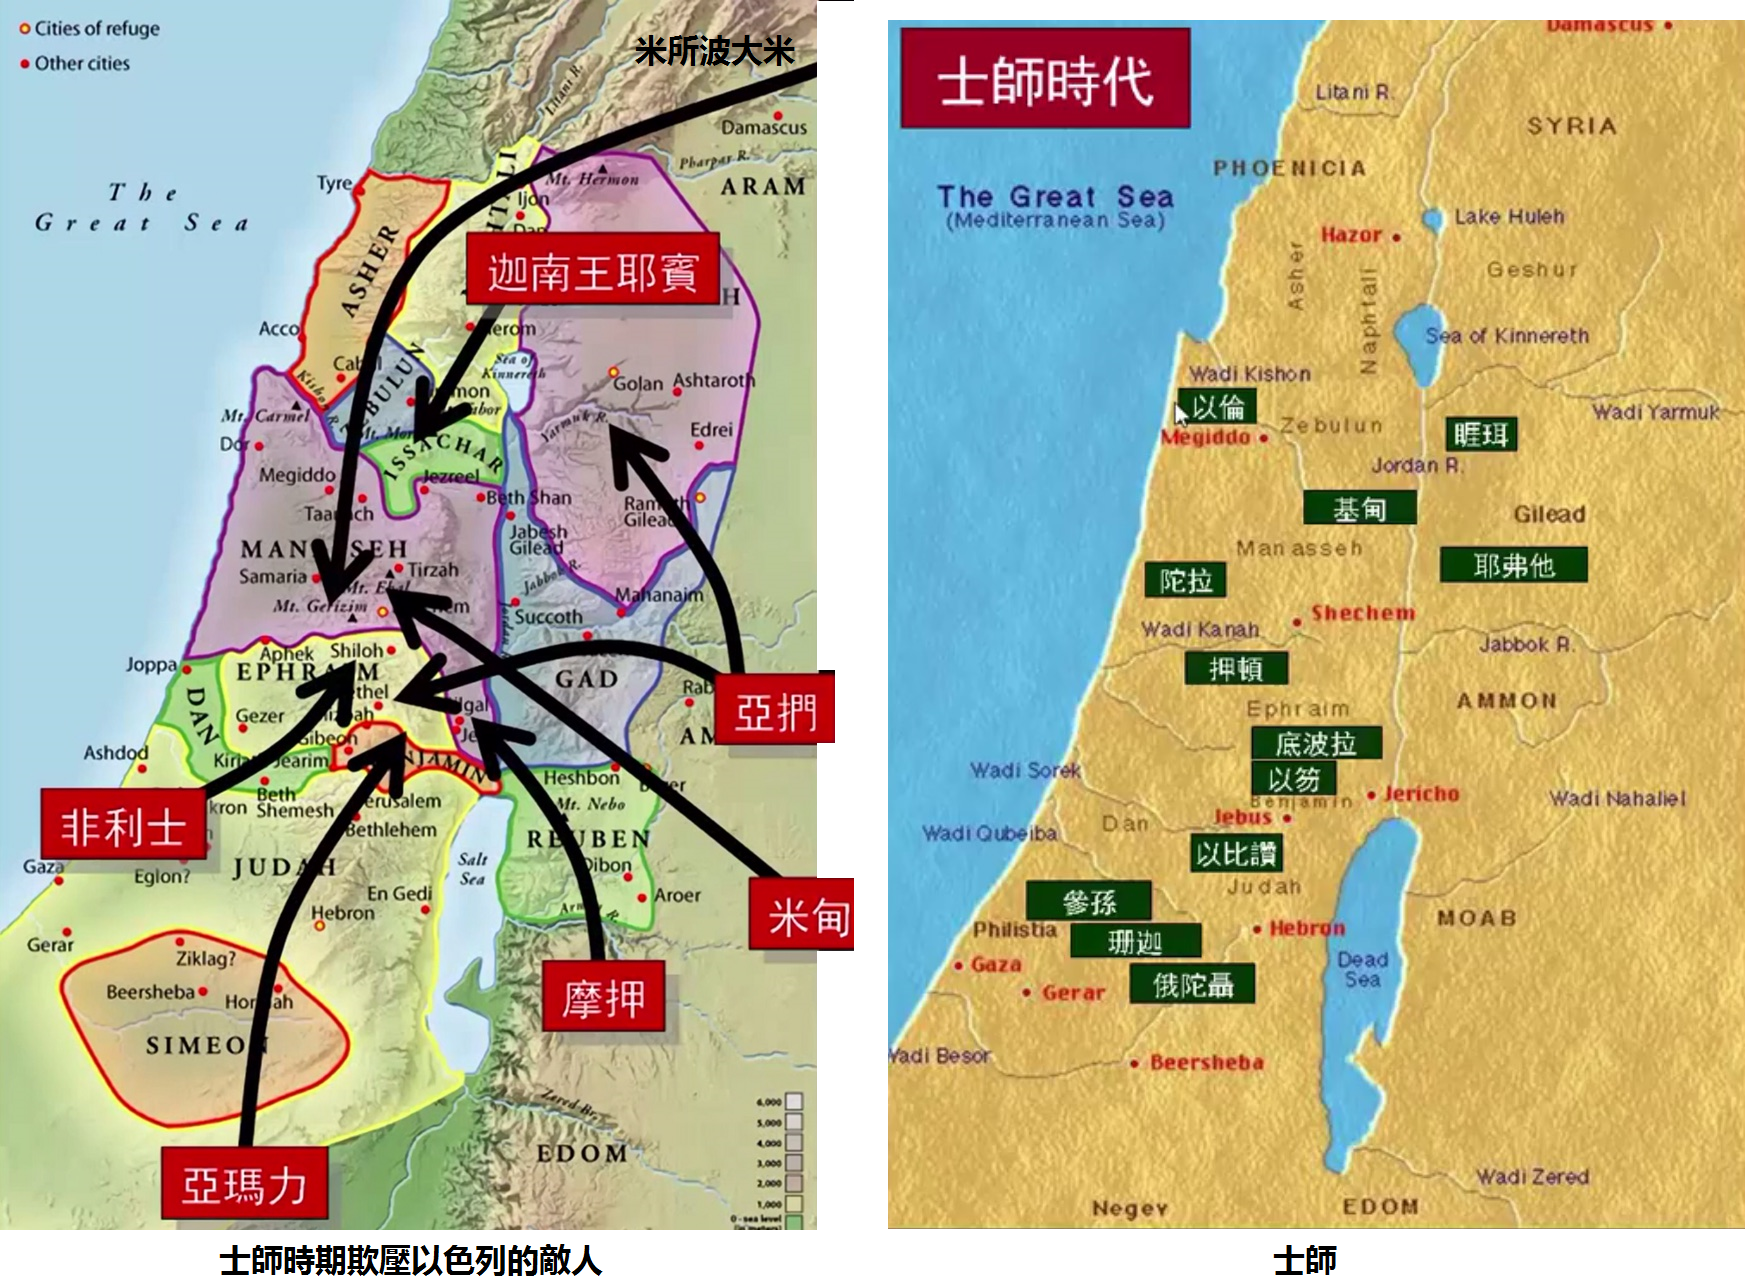
\includegraphics[width=7in]{BLiShiFigs/judge/shishiji}
	 \caption{士師時期}
	 \label{fig:1} 
	 \end{center}
	 \end{figure}
\begin{table}[h!]
\centering
\begin{tabular}{c|c|c|c|c}\hline
士師                 &所屬支派 & 敵人                     & 任職時間  &  聖經章節   \\\hline\hline
俄陀聶(基納斯兒子) &猶大     & 美索不達米亞王古珊利薩田 & 四十年    &  3:7-11     \\\hline
以笏 (基拉兒子)    & 便雅憫  & 摩押王伊磯倫             &  八十年   & 3:12-30\\\hline
珊迦 (亞拿兒子)    &         &非利士                    &           &3:31\\\hline
底波拉(拉比多妻)   &住在以法蓮山地 &夏瑣作王的迦南王耶賓 &四十年  &4,5\\\hline
巴拉(亞比挪菴的兒子)&拿弗他利的基低斯 &夏瑣作王的迦南王耶賓 &四十年  &4,5\\\hline
基甸,耶路巴力(約阿施兒子)&瑪拿西& 米甸&四十年  &6-8\\\hline
亞比米勒(耶路巴力兒子)& 瑪拿西& &三年  &9\\\hline
陀拉(普瓦兒子)& 以薩迦&&二十三年&10:1-2\\\hline
睚珥 &  基列（猶大，瑪拿西人女婿） &  &二十二年&10:3-5\\\hline
耶弗他&基列人 & 亞捫人& 六年 &10:6-12:7\\\hline
以比讚&伯利恆人 &&七年&12:8-10\\\hline
以倫&伯利恆人 &&十年&12:11-12\\\hline
押頓 (希列兒子) &以法蓮地的比拉頓人 &&八年&12:13-15\\\hline
參孫(瑪挪亞兒子)&但 &非利士人&二十年 &13-16\\\hline
\end{tabular}
\caption{士師}
\end{table}

%\newpage


%\vspace*{10mm} 



\subsection{俄陀聶（40年） 3:7-11}
   \begin{figure}[H]  
	 \begin{center}
	 \includegraphics[width=7in]{BLiShiFigs/judge/fivejudges}
	 \caption{俄陀聶,底波拉,睚珥,耶弗他}
	 \label{fig:1} 
	 \end{center}
	 \end{figure}

\begin{table}[H]
\centering
\begin{tabular}{p{2.7cm}|p{3.8cm}|p{1.5cm}|p{8.3cm}}\hline\hline
行惡&服侍古珊利薩田&呼求&俄陀聶\\\hline
以色列人行耶和華眼中看為惡的事，忘記耶和華他們的神，去侍奉諸巴力和亞舍拉，
&所以耶和華的怒氣向以色列人發作，就把他們交在美索不達米亞王古珊利薩田的手中。以色列人服侍古珊利薩田八年。
&以色列人呼求耶和華的時候，
&耶和華就為他們興起一位拯救者救他們，就是迦勒兄弟基納斯的兒子俄陀聶\footnote{書15:13-19，士1:11-15}。耶和華的靈降在他身上，他就做了以色列的士師，出去爭戰。耶和華將美索不達米亞王古珊利薩田交在他手中，他便勝了古珊利薩田。於是國中太平四十年。基納斯的兒子俄陀聶死了。\\\hline
 \end{tabular}
\caption{俄陀聶}
\end{table}

\subsection{以笏（80年）  3:12-30}
\subsubsection{摩押王伊磯倫占據棕樹城 3:12-15}
\begin{table}[H]
\centering
\begin{tabular}{p{2.5cm}|p{8.cm}|p{1.7cm}|p{3.5cm}}\hline\hline
行惡&摩押王伊磯倫&呼求&以笏\\\hline
以色列人又行耶和華眼中看為惡的事，
&耶和華就使摩押王伊磯倫強盛，攻擊以色列人。伊磯倫招聚亞捫人和亞瑪力人，去攻打以色列人，占據棕樹城。於是以色列人服侍摩押王伊磯倫十八年。
&以色列人呼求耶和華的時候，
&耶和華就為他們興起一位拯救者，就是便雅憫人基拉的兒子以笏。\\\hline
 \end{tabular}
\caption{行惡循环圈}
\end{table}

\subsubsection{刺殺摩押王伊磯倫 3:15-25}
\begin{wrapfigure}{r}{0.5\textwidth}
	 \begin{center}
	 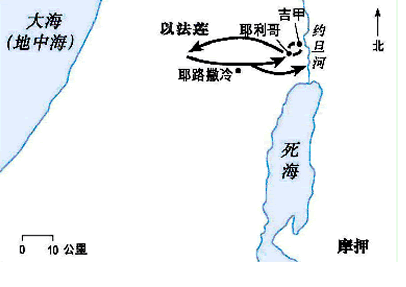
\includegraphics[width=4in]{BLiShiFigs/judge/yihu}
	 \caption{摩押王伊矶伦攻占耶利哥}
	 \label{fig:1} 
	 \end{center}
	 \end{wrapfigure}
他是左手便利的。以色列人託他送禮物給摩押王伊磯倫。以笏打了一把兩刃的劍，長一肘，帶在右腿上衣服裡面。他將禮物獻給摩押王伊磯倫，原來伊磯倫極其肥胖。以笏獻完禮物，便將抬禮物的人打發走了，自己卻從靠近吉甲鑿石之地回來，說：「王啊，我有一件機密事奏告你。」王說：「迴避吧！」於是左右侍立的人都退去了。以笏來到王面前，王獨自一人坐在涼樓上。以笏說：「我奉神的命報告你一件事。」王就從座位上站起來。以笏便伸左手，從右腿上拔出劍來，刺入王的肚腹，連劍把都刺進去了。劍被肥肉夾住，他沒有從王的肚腹拔出來，且穿通了後身。以笏就出到遊廊，將樓門盡都關鎖。以笏出來之後，王的僕人到了，看見樓門關鎖，就說：「他必是在樓上大解。」他們等煩了，見仍不開樓門，就拿鑰匙開了，不料，他們的主人已死，倒在地上。

\subsubsection{在以法蓮山地召集以色列人 3:26-27}
他們耽延的時候，以笏就逃跑了，經過鑿石之地，逃到西伊拉。到了，就在以法蓮山地吹角。以色列人隨著他下了山地，他在前頭引路，對他們說：「你們隨我來，因為耶和華已經把你們的仇敵摩押人交在你們手中。」

\subsubsection{制伏摩押國中太平 3:28-30}
於是他們跟著他下去，把守約旦河的渡口，不容摩押一人過去。 29 那時擊殺了摩押人約有一萬，都是強壯的勇士，沒有一人逃脫。這樣，摩押就被以色列人制伏了。國中太平八十年。	
	  
\subsection{珊迦 3:31}
以笏之後，有亞拿的兒子珊迦，他用趕牛的棍子打死六百非利士人。他也救了以色列人。

\subsection{底波和拉巴拉（40年） 4-5}
\subsubsection{迦南王耶賓欺壓以色列人 4:1-4}
\begin{table}[H]
\centering
\begin{tabular}{p{2.7cm}|p{8.cm}|p{1.7cm}|p{3.5cm}}\hline\hline
行惡&夏瑣王耶賓&呼求&底波拉\\\hline
以笏死後，以色列人又行耶和華眼中看為惡的事，
&耶和華就把他們付於在夏瑣做王的迦南王耶賓手中。他的將軍是西西拉，住在外邦人的夏羅設。耶賓王有鐵車九百輛，他大大欺壓以色列人二十年，
&以色列人就呼求耶和華。
&有一位女先知名叫底波拉，是拉比多的妻，當時做以色列的士師。\\\hline
 \end{tabular}
\caption{行惡循环圈}
\end{table}


\subsubsection{底波拉吩咐巴拉出战 4:5-10}
\begin{table}[H]
\centering
\begin{tabular}{p{11.7cm}|p{5.3cm}}\hline\hline
底波拉&巴拉\\\hline
她住在以法蓮山地拉瑪和伯特利中間，在底波拉的棕樹下，
&以色列人都上她那裡去聽判斷。\\\hline
她打發人從拿弗他利的基低斯將亞比挪菴的兒子巴拉召了來，對他說：「耶和華以色列的神吩咐你說：『你率領一萬拿弗他利和西布倫人上他泊山去。我必使耶賓的將軍西西拉率領他的車輛和全軍往基順河，到你那裡去。我必將他交在你手中。』」&巴拉說：「你若同我去，我就去；你若不同我去，我就不去。」\\\hline
底波拉說：「我必與你同去，只是你在所行的路上得不著榮耀，因為耶和華要將西西拉交在一個婦人手裡。」於是底波拉起來，與巴拉一同往基低斯去了。&巴拉就招聚西布倫人和拿弗他利人到基低斯，跟他上去的有一萬人。\\\hline
底波拉也同他上去。&\\\hline
 \end{tabular}
\caption{底波拉吩咐巴拉出战}
\end{table}



\subsubsection{摩西岳父後裔基尼人 4:11}
摩西岳父（內兄）何巴的後裔基尼人希百曾離開基尼族，到靠近基低斯撒拿音的橡樹旁支搭帳篷。

\subsubsection{巴拉底波拉戰敗西西拉 4:12-16}
\begin{table}[H]
\centering
\begin{tabular}{p{6.5cm}|p{3.98cm}|p{3.5cm}|p{2.5cm}}\hline\hline
西西拉&底波拉&巴拉&耶和華\\\hline
有人告訴西西拉說，亞比挪菴的兒子巴拉已經上他泊山了。西西拉就聚集所有的鐵車九百輛和跟隨他的全軍，從外邦人的夏羅設出來，到了基順河。
&底波拉對巴拉說：「你起來，今日就是耶和華將西西拉交在你手的日子。耶和華豈不在你前頭行嗎？」&於是巴拉下了他泊山，跟隨他有一萬人。&耶和華使西西拉和他一切車輛全軍潰亂，在巴拉面前被刀殺敗。\\\hline
西西拉下車步行逃跑。&&巴拉追趕車輛、軍隊，直到外邦人的夏羅設。&\\\hline
西西拉的全軍都倒在刀下，沒有留下一人。&&&\\\hline
 \end{tabular}
\caption{巴拉底波拉戰敗西西拉}
\end{table}


\subsubsection{雅億殺西西拉 4:17-24}
\begin{table}[H]
\centering
\begin{tabular}{p{8.5cm}|p{8.5cm}}\hline\hline
西西拉&雅億\\\hline
只有西西拉步行逃跑，到了基尼人希百之妻雅億的帳篷，因為夏瑣王耶賓與基尼人希百家和好。
&雅億出來迎接西西拉，對他說：「請我主進來，不要懼怕。」\\\hline
西西拉就進了她的帳篷。&雅億用被將他遮蓋。\\\hline
西西拉對雅億說：「我渴了，求你給我一點水喝。」&雅億就打開皮袋，給他奶子喝，仍舊把他遮蓋。\\\hline
西西拉又對雅億說：「請你站在帳篷門口，若有人來問你說有人在這裡沒有，你就說沒有。」西西拉疲乏沉睡。&希百的妻雅億取了帳篷的橛子，手裡拿著錘子，輕悄悄地到他旁邊，將橛子從他鬢邊釘進去，釘入地裡，\\\hline
西西拉就死了。&巴拉追趕西西拉的時候，雅億出來迎接他說：「來吧，我將你所尋找的人給你看。」\\\hline
他就進入帳篷，看見西西拉已經死了，倒在地上，橛子還在他鬢中。&這樣，神使迦南王耶賓被以色列人制伏了。從此以色列人的手越發有力，勝了迦南王耶賓，直到將他滅絕了。\\\hline
 \end{tabular}
\caption{雅億殺西西拉}
\end{table}



\subsubsection{底波拉巴拉作歌-赞美神 5:1-11}
\begin{table}[H]
\centering
\begin{tabular}{p{6.75cm}|p{10.750cm}}\hline\hline
\multicolumn{1}{c|}{赞美神}&\multicolumn{1}{c}{戰前的凄凉/戰后的赞美}\\\hline
\multirow{2}{6.9cm}{那時，底波拉和亞比挪菴的兒子巴拉作歌，說：「因為以色列中有軍長率領，百姓也甘心犧牲自己，你們應當頌讚耶和華。君王啊，要聽！王子啊，要側耳而聽！我要向耶和華歌唱，我要歌頌耶和華以色列的神。耶和華啊，你從西珥出來，由以東地行走，那時地震天漏，雲也落雨。山見耶和華的面就震動，西奈山見耶和華以色列神的面也是如此。}&在亞拿之子珊迦的時候，又在雅億的日子，大道無人行走，都是繞道而行。以色列中的官長停職，直到我底波拉興起，等我興起做以色列的母。以色列人選擇新神，爭戰的事就臨到城門，那時，以色列四萬人中豈能見藤牌槍矛呢？\\\cline{2-2}
&我心傾向以色列的首領，他們在民中甘心犧牲自己。你們應當頌讚耶和華！騎白驢的、坐繡花毯子的、行路的，你們都當傳揚。在遠離弓箭響聲打水之處，人必述說耶和華公義的作為，就是他治理以色列公義的作為。那時耶和華的民下到城門。\\\hline
\end{tabular}
\end{table} 

\subsubsection{底波拉巴拉作歌-称赞各支派 5:12-23}
\begin{table}[H]
\centering
\begin{tabular}{p{13.75cm}|p{3.750cm}}\hline\hline
\multicolumn{1}{c|}{参戰的人}&\multicolumn{1}{c}{神参戰}\\\hline
底波拉啊，興起，興起！你當興起，興起，唱歌！亞比挪菴的兒子巴拉啊，你當奮興，擄掠你的敵人！那時有餘剩的貴胄和百姓一同下來；耶和華降臨，為我攻擊勇士。有根本在亞瑪力人的地，從\textcolor{blue}{以法蓮}下來的；\textcolor{blue}{便雅憫}在民中跟隨你；有掌權的從\textcolor{blue}{瑪吉}下來；有持杖檢點民數的從\textcolor{blue}{西布倫}下來；以薩迦的首領與底波拉同來，\textcolor{blue}{以薩迦}怎樣，巴拉也怎樣。眾人都跟隨巴拉衝下平原。
&\multirow{4}{3.9cm}{星宿從天上爭戰，從其軌道攻擊西西拉。基順古河把敵人沖沒。我的靈啊，應當努力前行！那時壯馬馳驅，踢跳，奔騰。耶和華的使者說：『應當咒詛\textcolor{red}{米羅斯}，大大咒詛其中的居民，因為他們不來幫助耶和華，不來幫助耶和華攻擊勇士。』}\\\cline{1-1}
在\textcolor{blue}{魯本}的溪水旁，有心中定大志的。你為何坐在羊圈內聽群中吹笛的聲音呢？在\textcolor{blue}{魯本}的溪水旁，有心中設大謀的。\textcolor{blue}{基列}人安居在約旦河外。\textcolor{blue}{但}人為何等在船上？\textcolor{blue}{亞設}人在海口靜坐，在港口安居。&\\\cline{1-1}
\textcolor{blue}{西布倫}人是拼命敢死的，\textcolor{blue}{拿弗他利}人在田野的高處也是如此。&\\\cline{1-1}
君王都來爭戰。那時迦南諸王在米吉多水旁的他納爭戰，卻未得擄掠銀錢。&\\\hline
\end{tabular}
\end{table} 


\subsubsection{底波拉巴拉作歌-称赞雅億 5:24-27}
願基尼人希百的妻雅億比眾婦人多得福氣，比住帳篷的婦人更蒙福祉！西西拉求水，雅億給他奶子，用寶貴的盤子給他奶油。雅億左手拿著帳篷的橛子，右手拿著匠人的錘子，擊打西西拉，打傷他的頭，把他的鬢角打破穿通。西西拉在她腳前曲身仆倒，在她腳前曲身倒臥；在哪裡曲身，就在哪裡死亡。

\subsubsection{底波拉巴拉作歌-愿仇敵都滅亡 5:28-31}
「西西拉的母親從窗戶裡往外觀看，從窗櫺中呼叫說：『他的戰車為何耽延不來呢？他的車輪為何行得慢呢？』聰明的宮女安慰她(回答她)，她也自言自語地說：『他們莫非得財而分？每人得了一兩個女子。西西拉得了彩衣為擄物，得繡花的彩衣為掠物。這彩衣兩面繡花，乃是披在被擄之人頸項上的。』耶和華啊，願你的仇敵都這樣滅亡！願愛你的人如日頭出現，光輝烈烈！」這樣，國中太平四十年。


\subsection{基甸(耶路巴力40年) 6-8}
\begin{figure}[!htb]  
	 \begin{center}
	 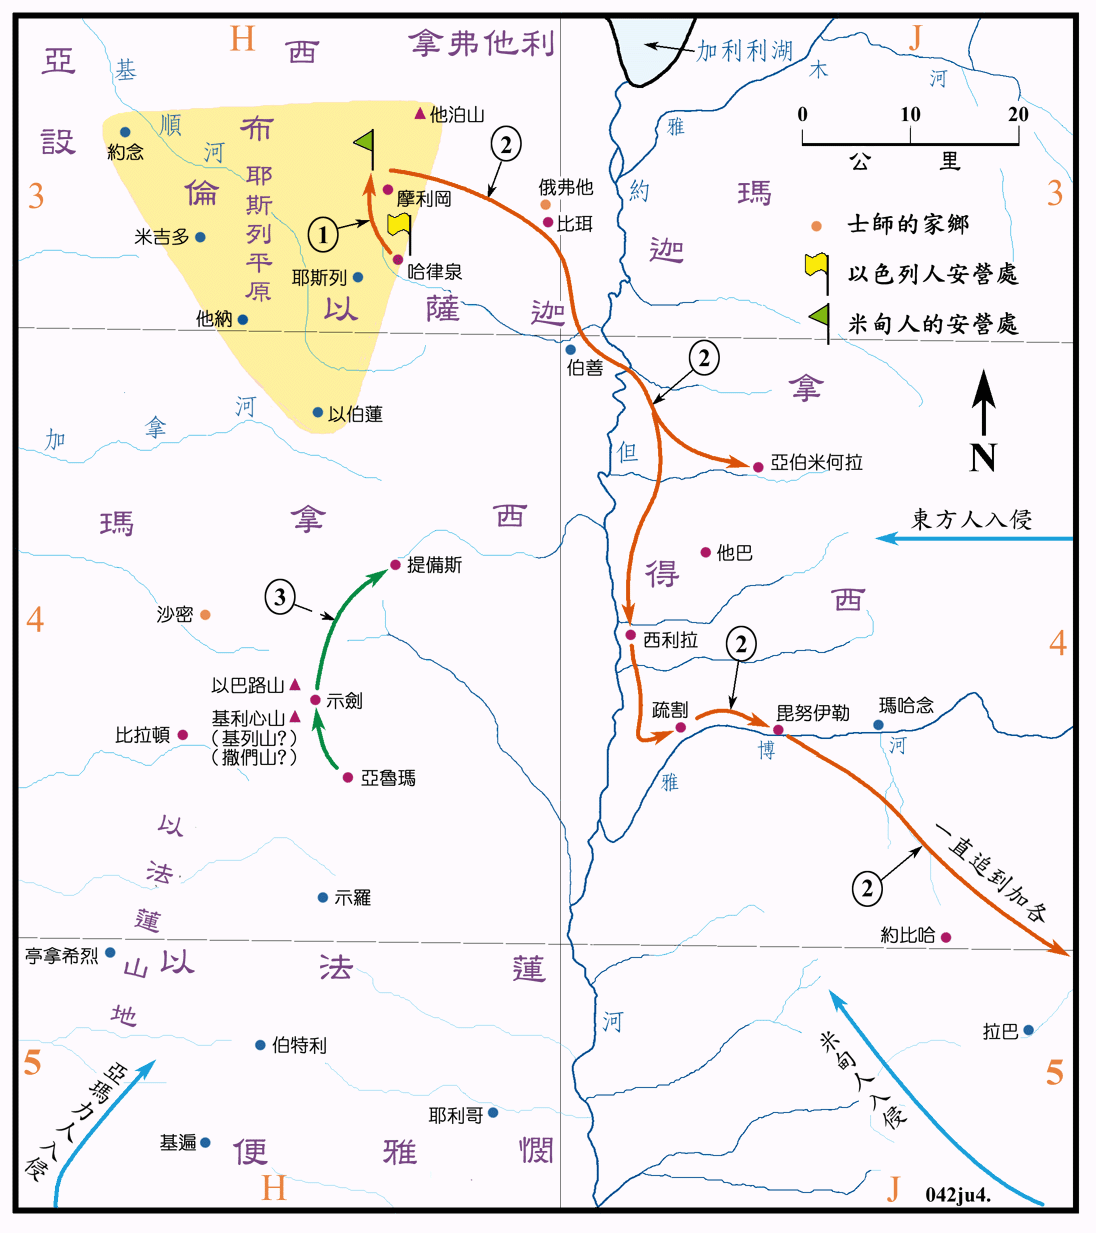
\includegraphics[width=7in]{BLiShiFigs/judge/jidian}
	 \caption{基甸,亞比米勒,陀拉}
	 \label{fig:1} 
	 \end{center}
	 \end{figure}
	
\subsubsection{以色列交在米甸人手裡七年 6:1-10} 
\begin{table}[H]
\centering
\begin{tabular}{p{0.89cm}|p{7.cm}|p{1.9cm}|p{6.5cm}}\hline\hline
行惡&米甸人&呼求&耶和華差遣先知\\\hline
以色列人又行耶和華眼中看為惡的事，
&耶和華就把他們交在米甸人手裡七年。米甸人壓制以色列人，以色列人因為米甸人，就在山中挖穴、挖洞，建造營寨。以色列人每逢撒種之後，米甸人、亞瑪力人和東方人都上來攻打他們，對著他們安營，毀壞土產，直到加沙，沒有給以色列人留下食物，牛、羊、驢也沒有留下。因為那些人帶著牲畜、帳篷來，像蝗蟲那樣多，人和駱駝無數，都進入國內，毀壞全地。
&以色列人因米甸人的緣故，極其窮乏，就呼求耶和華。以色列人因米甸人的緣故，呼求耶和華，
&耶和華就差遣先知到以色列人那裡，對他們說：「耶和華以色列的神如此說：『我曾領你們從埃及上來，出了為奴之家，救你們脫離埃及人的手，並脫離一切欺壓你們之人的手，把他們從你們面前趕出，將他們的地賜給你們。又對你們說：「我是耶和華你們的神。你們住在亞摩利人的地，不可敬畏他們的神。」你們竟不聽從我的話。』」\\\hline
 \end{tabular}
\caption{行惡循环圈}
\end{table}


\subsubsection{耶和華使者向基甸顯現 6:11-24} 
\begin{table}[H]
\centering
\begin{tabular}{p{6.5cm}|p{10.5cm}}\hline\hline
西西拉&雅億\\\hline
耶和華的使者到了俄弗拉，坐在亞比以謝族人約阿施的橡樹下。
&約阿施的兒子基甸正在酒榨那裡打麥子，為要防備米甸人。\\\hline
耶和華的使者向基甸顯現，對他說：「大能的勇士啊，耶和華與你同在！」 &基甸說：「主啊！耶和華若與我們同在，我們何至遭遇這一切事呢？我們的列祖不是向我們說，耶和華領我們從埃及上來嗎？他那樣奇妙的作為在哪裡呢？現在他卻丟棄我們，將我們交在米甸人手裡。」\\\hline
耶和華觀看基甸，說：「你靠著你這能力，去從米甸人手裡拯救以色列人。不是我差遣你去的嗎？」&基甸說：「主啊，我有何能拯救以色列人呢？我家在瑪拿西支派中是至貧窮的，我在我父家是至微小的。」\\\hline
耶和華對他說：「我與你同在，你就必擊打米甸人，如擊打一人一樣。」&基甸說：「我若在你眼前蒙恩，求你給我一個證據，使我知道與我說話的就是主。求你不要離開這裡，等我歸回將禮物帶來供在你面前。」\\\hline
主說：「我必等你回來。」&基甸去預備了一隻山羊羔，用一伊法細麵做了無酵餅，將肉放在筐內，把湯盛在壺中，帶到橡樹下，獻在使者面前。 \\\hline
神的使者吩咐基甸說：「將肉和無酵餅放在這磐石上，把湯倒出來。」&他就這樣行了。\\\hline
耶和華的使者伸出手內的杖，杖頭挨了肉和無酵餅，就有火從磐石中出來，燒盡了肉和無酵餅。耶和華的使者也就不見了。&基甸見他是耶和華的使者，就說：「哀哉！主耶和華啊，我不好了，因為我覿面看見耶和華的使者。」  \\\hline
耶和華對他說：「你放心，不要懼怕，你必不致死。」&於是基甸在那裡為耶和華築了一座壇，起名叫耶和華沙龍（耶和華賜平安）。這壇在亞比以謝族的俄弗拉，直到如今。 \\\hline
 \end{tabular}
\caption{耶和華使者向基甸顯現}
\end{table}

\subsubsection{基甸拆毀父親為巴力所築的壇 6:25-32}
\begin{table}[H]
\centering
\begin{tabular}{p{4.7cm}|p{2.6cm}|p{6.38cm}|p{3.3cm}}\hline\hline
耶和華&基甸&本城的人&約阿施\\\hline
\multirow{3}{4.7cm}{當那夜耶和華吩咐基甸說：「你取你父親的牛來，就是（和）那七歲的第二隻牛，並拆毀你父親為巴力所築的壇，砍下壇旁的木偶。在這磐石（保障）上整整齊齊地為耶和華你的神築一座壇，將第二隻牛獻為燔祭，用你所砍下的木偶做柴。」}
&\multirow{3}{2.8cm}{基甸就從他僕人中挑了十個人，照著耶和華吩咐他的行了。他因怕父家和本城的人，不敢在白晝行這事，就在夜間行了。}
&城裡的人清早起來，見巴力的壇拆毀，壇旁的木偶砍下，第二隻牛獻在新築的壇上，就彼此說：「這事是誰做的呢？」
&\multirow{3}{3.35cm}{約阿施回答站著攻擊他的眾人說：「你們是為巴力爭論嗎？你們要救他嗎？誰為他爭論，趁早將誰治死。巴力若果是神，有人拆毀他的壇，讓他為自己爭論吧！」}\\\cline{3-3}
&&他們訪查之後，就說：「這是約阿施的兒子基甸做的。」 &\\\cline{3-3}
&&城裡的人對約阿施說：「將你兒子交出來，好治死他，因為他拆毀了巴力的壇，砍下壇旁的木偶。」 &\\\hline
&&所以當日人稱基甸為耶路巴力，意思說：「他拆毀巴力的壇，讓巴力與他爭論。」&\\\hline
 \end{tabular}
\caption{基甸拆毀父親為巴力所築的壇}
\end{table}



\subsubsection{敌人聚集，基甸召集以色列人 6:33-35}
那時，米甸人、亞瑪力人和東方人都聚集過河，在耶斯列平原安營。耶和華的靈降在基甸身上，他就吹角，亞比以謝族都聚集跟隨他。他打發人走遍瑪拿西地，瑪拿西人也聚集跟隨他。又打發人去見亞設人、西布倫人、拿弗他利人，他們也都出來與他們會合。

\subsubsection{基甸以羊毛乾濕求問 6:36-40}
\begin{table}[H]
\centering
\begin{tabular}{p{9.5cm}|p{7.5cm}}\hline\hline
基甸&神\\\hline
基甸對神說：「你若果照著所說的話，藉我手拯救以色列人，我就把一團羊毛放在禾場上，若單是羊毛上有露水，別的地方都是乾的，我就知道你必照著所說的話，藉我手拯救以色列人。」 
&次日早晨基甸起來，見果然是這樣，將羊毛擠一擠，從羊毛中擰出滿盆的露水來。\\\hline
基甸又對神說：「求你不要向我發怒，我再說這一次，讓我將羊毛再試一次。但願羊毛是乾的，別的地方都有露水。」&這夜神也如此行，獨羊毛上是乾的，別的地方都有露水。\\\hline
 \end{tabular}
\caption{基甸以羊毛乾濕求問}
\end{table}


\subsubsection{神將人數從32000減為300人 7:1-8}
\begin{table}[H]
\centering
\begin{tabular}{p{5.cm}|p{8.cm}|p{3.9cm}}\hline\hline
基甸&神&以色列人\\\hline
耶路巴力就是基甸，他和一切跟隨的人早晨起來，在哈律泉旁安營。米甸營在他們北邊的平原，靠近摩利岡。
&耶和華對基甸說：「跟隨你的人過多，我不能將米甸人交在他們手中，免得以色列人向我誇大，說：『是我們自己的手救了我們。』現在你要向這些人宣告說：凡懼怕膽怯的，可以離開基列山回去。」&於是有二萬二千人回去，只剩下一萬。\\\hline
&耶和華對基甸說：「人還是過多。你要帶他們下到水旁，我好在那裡為你試試他們。我指點誰說，這人可以同你去，他就可以同你去；我指點誰說，這人不可同你去，他就不可同你去。」&\\\hline
基甸就帶他們下到水旁。&耶和華對基甸說：「凡用舌頭舔水，像狗舔的，要使他單站在一處；凡跪下喝水的，也要使他單站在一處。」&於是用手捧著舔水的有三百人，其餘的都跪下喝水。\\\hline
&耶和華對基甸說：「我要用這舔水的三百人拯救你們，將米甸人交在你手中。其餘的人都可以各歸各處去。」&這三百人就帶著食物和角。\\\hline
其餘的以色列人，基甸都打發他們各歸各的帳篷，只留下這三百人。米甸營在他下邊的平原裡。&&\\\hline
 \end{tabular}
\caption{神將人數從32000減為300人}
\end{table}







\subsubsection{基甸聽見敵人的夢和講解得信心 7:9-18}  
當那夜，耶和華吩咐基甸說：「起來，下到米甸營裡去，因我已將他們交在你手中。 10 倘若你怕下去，就帶你的僕人普拉下到那營裡去。你必聽見他們所說的，然後你就有膽量下去攻營。」

於是基甸帶著僕人普拉下到營旁。

米甸人、亞瑪力人和一切東方人都布散在平原，如同蝗蟲那樣多，他們的駱駝無數，多如海邊的沙。

基甸到了，就聽見一人將夢告訴同伴說：「我做了一夢，夢見一個大麥餅滾入米甸營中，到了帳幕，將帳幕撞倒，帳幕就翻轉傾覆了。」那同伴說：「這不是別的，乃是以色列人約阿施的兒子基甸的刀，神已將米甸和全軍都交在他的手中。」

基甸聽見這夢和夢的講解，就敬拜神，回到以色列營中，說：「起來吧！耶和華已將米甸的軍隊交在你們手中了。」

於是基甸將三百人分做三隊，把角和空瓶交在各人手裡，瓶內都藏著火把，吩咐他們說：「你們要看我行事，我到了營的旁邊怎樣行，你們也要怎樣行。我和一切跟隨我的人吹角的時候，你們也要在營的四圍吹角，喊叫說：『耶和華和基甸的刀！』」

\subsubsection{基甸用策警潰敵軍 7:19-23}  
基甸和跟隨他的一百人，在三更之初才換更的時候，來到營旁，就吹角，打破手中的瓶。三隊的人就都吹角，打破瓶子，左手拿著火把，右手拿著角，喊叫說：「耶和華和基甸的刀！」他們在營的四圍各站各的地方。全營的人都亂竄，三百人呐喊，使他們逃跑。三百人就吹角，耶和華使全營的人用刀互相擊殺，逃到西利拉的伯哈示他，直逃到靠近他巴的亞伯米何拉。以色列人就從拿弗他利、亞設和瑪拿西全地聚集來追趕米甸人。

\subsubsection{俄立西伊伯被誅 7:24-25}  
基甸打發人走遍以法蓮山地，說：「你們下來攻擊米甸人，爭先把守約旦河的渡口，直到伯巴拉。」於是以法蓮的眾人聚集，把守約旦河的渡口，直到伯巴拉。捉住了米甸人的兩個首領，一名俄立，一名西伊伯，將俄立殺在俄立磐石上，將西伊伯殺在西伊伯酒榨那裡。又追趕米甸人，將俄立和西伊伯的首級帶過約旦河，到基甸那裡。

\subsubsection{基甸平息以法連人的怒氣8:1-3）}  
以法蓮人對基甸說：「你去與米甸人爭戰，沒有招我們同去，為什麼這樣待我們呢？」他們就與基甸大大地爭吵。 2 基甸對他們說：「我所行的豈能比你們所行的呢？以法蓮拾取剩下的葡萄不強過亞比以謝所摘的葡萄嗎？ 3 神已將米甸人的兩個首領俄立和西伊伯交在你們手中。我所行的豈能比你們所行的呢？」基甸說了這話，以法蓮人的怒氣就消了。

\subsubsection{疏割人首領米甸拒绝帮助基甸 8:4-9}  
基甸和跟隨他的三百人到約旦河過渡，雖然疲乏，還是追趕。 5 基甸對疏割人說：「求你們拿餅來給跟隨我的人吃，因為他們疲乏了。我們追趕米甸人的兩個王西巴和撒慕拿。」 6 疏割人的首領回答說：「西巴和撒慕拿已經在你手裡，你使我們將餅給你的軍兵嗎？」 7 基甸說：「耶和華將西巴和撒慕拿交在我手之後，我就用野地的荊條和枳棘打傷你們。」 8 基甸從那裡上到毗努伊勒，對那裡的人也是這樣說。毗努伊勒人也與疏割人回答他的話一樣。 9 他向毗努伊勒人說：「我平平安安回來的時候，我必拆毀這樓。」
   
\subsubsection{捉住米甸的二王西巴和撒慕拿 8:10-12}
那時西巴和撒慕拿並跟隨他們的軍隊都在加各，約有一萬五千人，就是東方人全軍所剩下的，已經被殺約有十二萬拿刀的。 11 基甸就由挪巴和約比哈東邊，從住帳篷人的路上去，殺敗了米甸人的軍兵，因為他們坦然無懼。 12 西巴和撒慕拿逃跑，基甸追趕他們，捉住米甸的二王西巴和撒慕拿，驚散全軍。

\subsubsection{基甸殺了疏割城裡的人 8:13-17}
約阿施的兒子基甸由希列斯坡從陣上回來， 14 捉住疏割的一個少年人，問他疏割的首領長老是誰，他就將首領長老七十七個人的名字寫出來。 15 基甸到了疏割，對那裡的人說：「你們從前譏誚我說：『西巴和撒慕拿已經在你手裡，你使我們將餅給跟隨你的疲乏人嗎？』現在西巴和撒慕拿在這裡！」 16 於是捉住那城內的長老，用野地的荊條和枳棘責打(指教)疏割人。 17 又拆了毗努伊勒的樓，殺了那城裡的人。

\subsubsection{西巴撒慕拿被誅 8:18-21}
基甸問西巴和撒慕拿說：「你們在他泊山所殺的人是什麼樣式？」回答說：「他們好像你，各人都有王子的樣式。」 19 基甸說：「他們是我同母的弟兄，我指著永生的耶和華起誓，你們從前若存留他們的性命，我如今就不殺你們了。」 20 於是對他的長子益帖說：「你起來殺他們。」但益帖因為是童子，害怕，不敢拔刀。 21 西巴和撒慕拿說：「你自己起來殺我們吧！因為人如何，力量也是如何。」基甸就起來，殺了西巴和撒慕拿，奪獲他們駱駝項上戴的月牙圈。

\subsubsection{基甸治理以色列人 8:22-27}
 以色列人對基甸說：「你既救我們脫離米甸人的手，願你和你的兒孫管理我們。」 23 基甸說：「我不管理你們，我的兒子也不管理你們，唯有耶和華管理你們。」 24 基甸又對他們說：「我有一件事求你們，請你們各人將所奪的耳環給我。」原來仇敵是以實瑪利人，都是戴金耳環的。 25 他們說：「我們情願給你。」就鋪開一件外衣，各人將所奪的耳環丟在其上。 26 基甸所要出來的金耳環重一千七百舍客勒金子；此外，還有米甸王所戴的月環、耳墜和所穿的紫色衣服，並駱駝項上的金鏈子。 27 基甸以此製造了一個以弗得，設立在本城俄弗拉。後來以色列人拜那以弗得行了邪淫，這就做了基甸和他全家的網羅。 

\subsubsection{基甸去世 8:28-35}
這樣，米甸人被以色列人制伏了，不敢再抬頭。基甸還在的日子，國中太平四十年。

29 約阿施的兒子耶路巴力回去，住在自己家裡。 30 基甸有七十個親生的兒子，因為他有許多的妻。 31 他的妾住在示劍，也給他生了一個兒子，基甸與他起名叫亞比米勒。 32 約阿施的兒子基甸年紀老邁而死，葬在亞比以謝族的俄弗拉，在他父親約阿施的墳墓裡。

33 基甸死後，以色列人又去隨從諸巴力行邪淫，以巴力比利土為他們的神。 34 以色列人不記念耶和華他們的神，就是拯救他們脫離四圍仇敵之手的， 35 也不照著耶路巴力（就是基甸）向他們所施的恩惠厚待他的家。

\subsection{亞比米勒(3年) 9}
\subsubsection{亞比米勒殺基甸眾子 9:1-6}
\begin{table}[H]
\centering
\begin{tabular}{p{8.5cm}|p{2cm}|p{6cm}}\hline\hline
亞比米勒&眾母舅&示劍人\\\hline
耶路巴力的兒子亞比米勒到了示劍見他的眾母舅，對他們和他外祖全家的人說：「請你們問示劍的眾人說，是耶路巴力的眾子七十人都管理你們好呢，還是一人管理你們好呢？你們又要記念我是你們的骨肉。」 
&他的眾母舅便將這一切話為他說給示劍人聽，&示劍人的心就歸向亞比米勒。他們說：「他原是我們的弟兄。」就從巴力比利土的廟中取了七十舍客勒銀子給亞比米勒。\\\hline
亞比米勒用以雇了些匪徒跟隨他。他往俄弗拉到他父親的家，將他弟兄耶路巴力的眾子七十人都殺在一塊磐石上；只剩下耶路巴力的小兒子約坦，因為他躲藏了。&&示劍人和米羅人都一同聚集，往示劍橡樹旁的柱子那裡，立亞比米勒為王。\\\hline
 \end{tabular}
\caption{亞比米勒殺基甸眾子}
\end{table}

\subsubsection{約坦在基利心山上用比喻勸說示劍人 9:7-21}    
\begin{table}[H]
\centering
\begin{tabular}{p{2.85cm}|p{8.cm}|p{6.2cm}}\hline\hline
亞比米勒&眾母舅&示劍人\\\hline
\multirow{4}{2.85cm}{有人將這事告訴約坦，他就去站在基利心山頂上，向眾人大聲喊叫說：「示劍人哪，你們要聽我的話，神也就聽你們的話。} 
&有一時樹木要膏一樹為王，管理它們，就去對橄欖樹說：『請你做我們的王。』橄欖樹回答說：『我豈肯止住供奉神和尊重人的油，飄搖在眾樹之上呢？』 &\multirow{4}{6.25cm}{現在你們立亞比米勒為王，若按誠實、正直善待耶路巴力和他的全家，這就是酬他的勞。從前我父冒死為你們爭戰，救了你們脫離米甸人的手。你們如今起來攻擊我的父家，將他眾子七十人殺在一塊磐石上，又立他婢女所生的兒子亞比米勒為示劍人的王，他原是你們的弟兄。你們如今若按誠實、正直待耶路巴力和他的家，就可因亞比米勒得歡樂，他也可因你們得歡樂。不然，願火從亞比米勒發出，燒滅示劍人和米羅眾人；又願火從示劍人和米羅人中出來，燒滅亞比米勒。」} \\\cline{2-2}
&樹木對無花果樹說：『請你來做我們的王。』無花果樹回答說：『我豈肯止住所結甜美的果子，飄搖在眾樹之上呢？』&\\\cline{2-2}
&樹木對葡萄樹說：『請你來做我們的王。』葡萄樹回答說：『我豈肯止住使神和人喜樂的新酒，飄搖在眾樹之上呢？』&\\\cline{2-2}
&眾樹對荊棘說：『請你來做我們的王。』荊棘回答說：『你們若誠誠實實地膏我為王，就要投在我的蔭下。不然願火從荊棘裡出來燒滅黎巴嫩的香柏樹。』 &\\\hline
約坦因怕他弟兄亞比米勒就逃跑來到比珥住在那裡&&\\\hline
 \end{tabular}
\caption{亞比米勒殺基甸眾子}
\end{table}  


\subsubsection{示劍人背叛亞比米勒 9:22-25}
亞比米勒管理以色列人三年。神使惡魔降在亞比米勒和示劍人中間，示劍人就以詭詐待亞比米勒。這是要叫耶路巴力七十個兒子所受的殘害歸於他們的哥哥亞比米勒，又叫那流他們血的罪歸於幫助他殺弟兄的示劍人。示劍人在山頂上設埋伏，等候亞比米勒，凡從他們那裡經過的人，他們就搶奪。有人將這事告訴亞比米勒。

\subsubsection{迦勒謀攻亞比米勒 9:26-29}
\begin{table}[H]
\centering
\begin{tabular}{p{8.85cm}|p{8.2cm}}\hline\hline
迦勒和他的弟兄&示劍人\\\hline
以別的兒子迦勒和他的弟兄來到示劍，
&示劍人都信靠他。示劍人出城到田間去，摘下葡萄，踹酒，設擺筵宴，進他們神的廟中吃喝，咒詛亞比米勒。\\\hline
以別的兒子迦勒說：「亞比米勒是誰，示劍是誰，使我們服侍他呢？他不是耶路巴力的兒子嗎？他的幫手不是西布勒嗎？你們可以服侍示劍的父親哈抹的後裔。我們為何服侍亞比米勒呢？唯願這民歸我的手下，我就除掉亞比米勒。」迦勒又對亞比米勒說：「增添你的軍兵出來吧！」&\\\hline
 \end{tabular}
\caption{迦勒謀攻亞比米勒}
\end{table}  


\subsubsection{亞比米勒擊敗迦勒 9:30-45}
邑宰西布勒聽見以別的兒子迦勒的話，就發怒，悄悄地打發人去見亞比米勒，說：「以別的兒子迦勒和他的弟兄到了示劍，煽惑城中的民攻擊你。現在你和跟隨你的人今夜起來，在田間埋伏。到早晨太陽一出，你就起來闖城。迦勒和跟隨他的人出來攻擊你的時候，你便向他們見機而做。」
於是，亞比米勒和跟隨他的眾人夜間起來，分做四隊，埋伏等候示劍人。以別的兒子迦勒出去，站在城門口，亞比米勒和跟隨他的人從埋伏之處起來。迦勒看見那些人，就對西布勒說：「看哪，有人從山頂上下來了。」西布勒說：「你看見山的影子，以為是人。」迦勒又說：「看哪，有人從高處下來，又有一隊從米惡尼尼橡樹的路上而來。」西布勒對他說：「你曾說：『亞比米勒是誰，叫我們服侍他？』你所誇的口在哪裡呢？這不是你所藐視的民嗎？你現在出去，與他們交戰吧！」於是迦勒率領示劍人出去，與亞比米勒交戰。亞比米勒追趕迦勒，迦勒在他面前逃跑，有許多受傷仆倒的，直到城門。

41 亞比米勒住在亞魯瑪。西布勒趕出迦勒和他弟兄，不准他們住在示劍。次日，民出到田間，有人告訴亞比米勒。 43 他就把他的人分做三隊，埋伏在田間，看見示劍人從城裡出來，就起來擊殺他們。 44 亞比米勒和跟隨他的一隊向前闖去，站在城門口。那兩隊直闖到田間，擊殺了眾人。 45 亞比米勒整天攻打城，將城奪取，殺了其中的居民，將城拆毀，撒上了鹽。

\subsubsection{焚示劍樓 9:46-49}
示劍樓的人聽見了，就躲入巴力比利土廟的衛所。有人告訴亞比米勒說，示劍樓的人都聚在一處， 48 亞比米勒和跟隨他的人就都上撒們山。亞比米勒手拿斧子，砍下一根樹枝，扛在肩上，對跟隨他的人說：「你們看我所行的，也當趕緊照樣行。」眾人就各砍一枝，跟隨亞比米勒，把樹枝堆在衛所的四圍，放火燒了衛所，以致示劍樓的人都死了，男女約有一千。

\subsubsection{亞比米勒在提備斯被婦人所殺 9:50-57}  
亞比米勒到提備斯，向提備斯安營，就攻取了那城。城中有一座堅固的樓，城裡的眾人，無論男女，都逃進樓去，關上門，上了樓頂。亞比米勒到了樓前攻打，挨近樓門，要用火焚燒。有一個婦人把一塊上磨石拋在亞比米勒的頭上，打破了他的腦骨。他就急忙喊叫拿他兵器的少年人，對他說：「拔出你的刀來殺了我吧！免得人議論我說：『他為一個婦人所殺。』」於是少年人把他刺透，他就死了。以色列人見亞比米勒死了，便各回自己的地方去了。這樣，神報應亞比米勒向他父親所行的惡，就是殺了弟兄七十個人的惡。示劍人的一切惡，神也都報應在他們頭上，耶路巴力的兒子約坦的咒詛歸到他們身上了。


\subsection{陀拉(23年) 10:1-2}
亞比米勒以後，有以薩迦人朵多的孫子、普瓦的兒子陀拉興起，拯救以色列人。他住在以法蓮山地的沙密。 2 陀拉做以色列的士師二十三年，就死了，葬在沙密。

\subsection{睚珥(22年) 10:3-5}
在他以後有基列人睚珥\footnote{士10:3-5，代上2:21-23，申3:13-15}興起，做以色列的士師二十二年。他有三十個兒子，騎著三十匹驢駒。他們有三十座城邑，叫做哈倭特睚珥，直到如今，都是在基列地。睚珥死了，就葬在加們。

	 
\subsection{耶弗他(6年)  10:6-12:7}
%\subsubsection{以色列人事奉假神 10:6-9}
\subsubsection{以色列人哀求耶和華 10:6-16}
\begin{table}[H]
\centering
\begin{tabular}{p{2.7cm}|p{4.2cm}|p{8.8cm}|p{1.2cm}}\hline\hline
離棄耶和華&受亞捫人欺&哀求耶和華&神眷顾\\\hline
以色列人又行耶和華眼中看為惡的事，去侍奉諸巴力和亞斯她錄，並亞蘭的神、西頓的神、摩押的神、亞捫人的神、非利士人的神，離棄耶和華，不侍奉他。
&耶和華的怒氣向以色列人發作，就把他們交在非利士人和亞捫人的手中。從那年起，他們擾害欺壓約旦河那邊住亞摩利人之基列地的以色列人，共有十八年。亞捫人又渡過約旦河去攻打猶大和便雅憫並以法蓮族，以色列人就甚覺窘迫。
&以色列人哀求耶和華說：「我們得罪了你！因為離棄了我們神，去侍奉諸巴力。」耶和華對以色列人說：「我豈沒有救過你們脫離埃及人、亞摩利人、亞捫人和非利士人嗎？西頓人、亞瑪力人、馬雲人也都欺壓你們，你們哀求我，我也拯救你們脫離他們的手。你們竟離棄我，侍奉別神，所以我不再救你們了。你們去哀求所選擇的神！你們遭遇急難的時候，讓他救你們吧！」以色列人對耶和華說：「我們犯罪了，任憑你隨意待我們吧，只求你今日拯救我們！」以色列人就除掉他們中間的外邦神，侍奉耶和華。
&耶和華因以色列人受的苦難，就心中擔憂。\\\hline
 \end{tabular}
\caption{作恶循环圈}
\end{table}  
 

\subsubsection{亞捫人聚集，安營在基列 10:17-18}
當時亞捫人聚集，安營在基列。以色列人也聚集，安營在米斯巴。基列的民和眾首領彼此商議說：「誰能先去攻打亞捫人，誰必做基列一切居民的領袖。」    

\subsubsection{妓女的兒子-耶弗他 11:1-3}
基列人耶弗他是個大能的勇士，是妓女的兒子。耶弗他是基列所生的。基列的妻也生了幾個兒子，他妻所生的兒子長大了，就趕逐耶弗他，說：「你不可在我們父家承受產業，因為你是妓女的兒子。」耶弗他就逃避他的弟兄，去住在陀伯地，有些匪徒到他那裡聚集，與他一同出入。

\subsubsection{民立耶弗他做首領 11:4-11}
過了些日子，亞捫人攻打以色列。亞捫人攻打以色列的時候，基列的長老到陀伯地去，要叫耶弗他回來，對耶弗他說：「請你來做我們的元帥，我們好與亞捫人爭戰。」耶弗他回答基列的長老說：「從前你們不是恨我，趕逐我出離父家嗎？現在你們遭遇急難為何到我這裡來呢？」基列的長老回答耶弗他說：「現在我們到你這裡來，是要你同我們去，與亞捫人爭戰。你可以做基列一切居民的領袖。」耶弗他對基列的長老說：「你們叫我回去，與亞捫人爭戰，耶和華把他交給我，我可以做你們的領袖嗎？」基列的長老回答耶弗他說：「有耶和華在你我中間做見證，我們必定照你的話行。」於是耶弗他同基列的長老回去，百姓就立耶弗他做領袖，做元帥。耶弗他在米斯巴將自己的一切話陳明在耶和華面前。

\subsubsection{耶弗他與亞捫人談判失敗 11:12-28}  
\begin{table}[H]
\centering
\begin{tabular}{p{12.3cm}|p{4.7cm}}\hline\hline
迦勒和他的弟兄&示劍人\\\hline
耶弗他打發使者去見亞捫人的王，說：「你與我有什麼相干，竟來到我國中攻打我呢？」
&亞捫人的王回答耶弗他的使者說：「因為以色列人從埃及上來的時候占據我的地，從亞嫩河到雅博河，直到約旦河。現在你要好好地將這地歸還吧！」\\\hline
耶弗他又打發使者去見亞捫人的王對他說：「耶弗他如此說：『以色列人並沒有占據摩押地和亞捫人的地。以色列人從埃及上來乃是經過曠野到紅海，來到加低斯就打發使者去見\textcolor{blue}{以東王}說：「求你容我從你的地經過。」以東王卻不應允。
&但亞捫人的王不肯聽耶弗他打發人說的話。\\\cline{1-1}
又照樣打發使者去見\textcolor{blue}{摩押王}，他也不允准。以色列人就住在加低斯。他們又經過曠野，繞著以東和摩押地，從摩押地的東邊過來，在亞嫩河邊安營，並沒有入摩押的境內，因為亞嫩河是摩押的邊界。&\\\cline{1-1}
以色列人打發使者去見\textcolor{blue}{亞摩利王西宏}，就是希實本的王，對他說：「求你容我們從你的地經過，往我們自己的地方去。」西宏卻不信服以色列人，不容他們經過他的境界，乃招聚他的眾民在雅雜安營，與以色列人爭戰。耶和華以色列的神將西宏和他的眾民都交在以色列人手中，以色列人就擊殺他們，得了亞摩利人的全地，從亞嫩河到雅博河，從曠野直到約旦河。耶和華以色列的神在他百姓以色列面前趕出亞摩利人，&\\\cline{1-1}
你竟要得他們的地嗎？你的神基抹所賜你的地，你不是得為業嗎？耶和華我們的神在我們面前所趕出的人，我們就得他的地。難道你比摩押王西撥的兒子巴勒還強嗎？他曾與以色列人爭競，或是與他們爭戰嗎？以色列人住希實本和屬希實本的鄉村，亞羅珥和屬亞羅珥的鄉村，並沿亞嫩河的一切城邑，已經有三百年了。在這三百年之內，你們為什麼沒有取回這些地方呢？原來我沒有得罪你，你卻攻打我，惡待我。願審判人的耶和華今日在以色列人和亞捫人中間判斷是非！』」&\\\hline
 \end{tabular}
\caption{耶弗他與亞捫人談判失敗}
\end{table}  


\subsubsection{耶弗他許願,殺敗亞捫人 11:29-33}  
耶和華的靈降在耶弗他身上，他就經過基列和瑪拿西，來到基列的米斯巴，又從米斯巴來到亞捫人那裡。耶弗他就向耶和華許願，說：「你若將亞捫人交在我手中，我從亞捫人那裡平平安安回來的時候，無論什麼人，先從我家門出來迎接我，就必歸你，我也必將他獻上為燔祭。」

於是耶弗他往亞捫人那裡去，與他們爭戰。耶和華將他們交在他手中，他就大大殺敗他們，從亞羅珥到米匿，直到亞備勒基拉明，攻取了二十座城。這樣，亞捫人就被以色列人制伏了。

\subsubsection{耶弗他回米斯巴獻女兒為祭 11:34-40}
\begin{table}[H]
\centering
\begin{tabular}{p{6.5cm}|p{10.6cm}}\hline\hline
迦勒和他的弟兄&示劍人\\\hline
耶弗他回米斯巴到了自己的家，
&不料，他女兒拿著鼓跳舞出來迎接他，是他獨生的，此外無兒無女。\\\hline
耶弗他看見她就撕裂衣服說：「哀哉！我的女兒啊，你使我甚是愁苦叫我作難了！因為我已經向耶和華開口許願不能挽回。」&他女兒回答說：「父啊，你既向耶和華開口，就當照你口中所說的向我行，因耶和華已經在仇敵亞捫人身上為你報仇。」又對父親說：「有一件事求你允准，容我去兩個月，與同伴在山上，好哀哭我終為處女。」\\\hline
耶弗他說：「你去吧！」就容她去兩個月。&她便和同伴去了在山上為她終為處女哀哭。兩月已滿她回到父親那裡，\\\hline
父親就照所許的願向她行了。&女兒終身沒有親近男子。\\\hline
此後以色列中有個規矩，&每年以色列的女子去為基列人耶弗他的女兒哀哭四天。\\\hline
 \end{tabular}
\caption{耶弗他回米斯巴獻女兒為祭}
\end{table}  


\subsubsection{耶弗他擊殺以法蓮人四萬二千人 12:1-6} 
\begin{table}[H]
\centering
\begin{tabular}{p{6.4cm}|p{6.6cm}|p{3.8cm}}\hline
基列人&以法蓮人&耶弗他\\\hline
&以法蓮人聚集，到了北方，對耶弗他說：「你去與亞捫人爭戰，為什麼沒有招我們同去呢？我們必用火燒你和你的房屋。」&\multirow{5}{4cm}{耶弗他對他們說"我和我的民與亞捫人大大爭戰,我招你們來,你們竟沒有來救我脫離他們的手。我見你們不來救我,我就拼命前去攻擊亞捫人，耶和華將他們交在我手中。你們今日為什麼上我這裡來攻打我呢?"於是耶弗他招聚基列人與以法蓮人爭戰。}\\\cline{1-2}
基列人擊殺以法蓮人，是因他們說「你們基列人在以法蓮瑪拿西中間，不過是以法蓮逃亡的人」。基列人把守約旦河的渡口，不容以法蓮人過去。&
以法蓮逃走的人若說：「容我過去」，& \\\cline{1-2}
基列人就問他說：「你是以法蓮人不是？」&
他若說：「不是」，&\\\cline{1-2}
就對他說：「你說示播列。」&
以法蓮人因為咬不真字音便說：「西播列。」&\\\cline{1-2}
基列人就將他拿住，殺在約旦河的渡口。&
那時以法蓮人被殺的有四萬二千人。&\\\hline
 \end{tabular}
\caption{耶弗他擊殺以法蓮人四萬二千人}
\end{table}  

 

\subsubsection{耶弗他卒 12:7}
耶弗他做以色列的士師六年。基列人耶弗他死了，葬在基列的一座城裡。


\subsection{以比讚（7年） 12:8-10}
耶弗他以後，有伯利恆人以比讚做以色列的士師。他有三十個兒子，三十個女兒。女兒都嫁出去了。他給眾子從外鄉娶了三十個媳婦。他做以色列的士師七年。以比讚死了，葬在伯利恆。

\subsection{以倫（10年） 12:11-12}
以比讚之後，有西布倫人以倫做以色列的士師十年。西布倫人以倫死了，葬在西布倫地的亞雅崙。

\subsection{押頓（8年） 12:13-15}
以倫之後，有比拉頓人希列的兒子押頓做以色列的士師。 他有四十個兒子，三十個孫子，騎著七十匹驢駒。押頓做以色列的士師八年。 比拉頓人希列的兒子押頓死了，葬在以法蓮地的比拉頓，在亞瑪力人的山地。

\subsection{參孫（20年） 13-16}
   \begin{figure}[!htb]  
	 \begin{center}
	 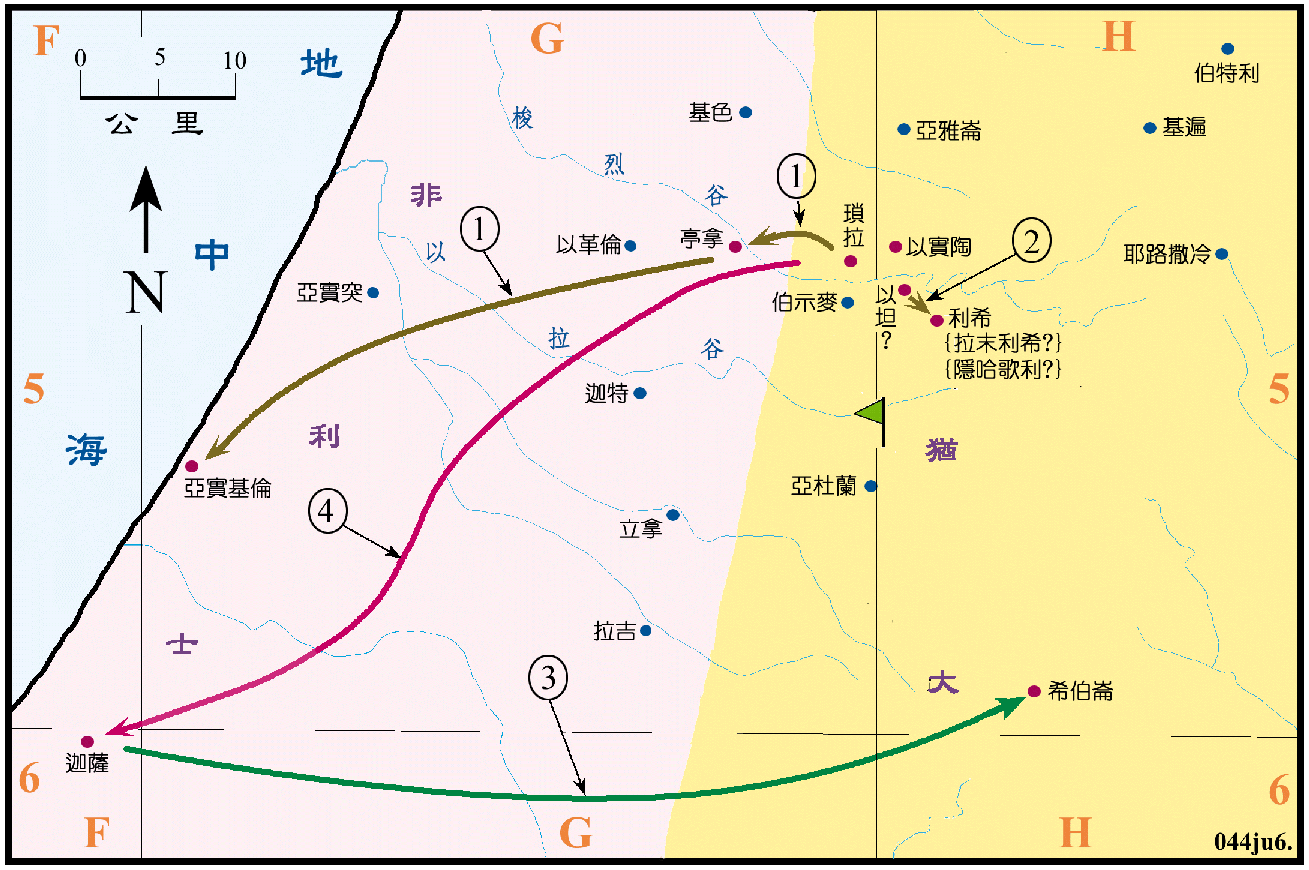
\includegraphics[width=7in]{BLiShiFigs/judge/cansun}
	 \caption{參孫}
	 \label{fig:1} 
	 \end{center}
	 \end{figure}

\subsubsection{為非利士人所制四十年 13:1}
以色列人又行耶和華眼中看為惡的事，耶和華將他們交在非利士人手中四十年。

\subsubsection{瑪挪亞妻見天使预言生子 13:2-7}
那時，有一個瑣拉人，是屬但族的，名叫瑪挪亞。他的妻不懷孕，不生育。耶和華的使者向那婦人顯現，對她說：「向來你不懷孕，不生育，如今你必懷孕生一個兒子。所以你當謹慎，清酒濃酒都不可喝，一切不潔之物也不可吃。你必懷孕生一個兒子，不可用剃頭刀剃他的頭，因為這孩子一出胎就歸神做拿細耳人。他必起首拯救以色列人脫離非利士人的手。」婦人就回去對丈夫說：「有一個神人到我面前來，他的相貌如神使者的相貌，甚是可畏。我沒有問他從哪裡來，他也沒有將他的名告訴我，卻對我說：『你要懷孕生一個兒子，所以清酒濃酒都不可喝，一切不潔之物也不可吃。因為這孩子從出胎一直到死，必歸神做拿細耳人。』」

\subsubsection{瑪挪亞與妻見天使 13:8-23}
\begin{table}[H]
\centering
\begin{tabular}{p{7.cm}|p{6.6cm}|p{3.4cm}}\hline
瑪挪亞&神的使者&瑪挪亞妻\\\hline
瑪挪亞就祈求耶和華說：「主啊，求你再差遣那神人到我們這裡來，好指教我們怎樣待這將要生的孩子。」&神應允瑪挪亞的話。&婦人正坐在田間的時候，\\\hline
&神的使者又到她那裡，& \\\hline
她丈夫瑪挪亞卻沒有同她在一處。&&婦人急忙跑去告訴丈夫說"那日到我面前來的人又向我顯現"\\\hline
瑪挪亞起來，跟隨他的妻來到那人面前，對他說：「與這婦人說話的就是你嗎？」&
他說：「是我。」&\\\hline
瑪挪亞說：「願你的話應驗！我們當怎樣待這孩子，他後來當怎樣呢？」&
耶和華的使者對瑪挪亞說：「我告訴婦人的一切事她都當謹慎。葡萄樹所結的都不可吃，清酒濃酒都不可喝，一切不潔之物也不可吃。凡我所吩咐的她都當遵守。」&\\\hline
瑪挪亞對耶和華的使者說：「求你容我們款留你，好為你預備一隻山羊羔。」&耶和華的使者對瑪挪亞說：「你雖然款留我，我卻不吃你的食物；你若預備燔祭，就當獻於耶和華。」&\\\hline
原來瑪挪亞不知道他是耶和華的使者。瑪挪亞對耶和華的使者說：「請將你的名告訴我，到你話應驗的時候，我們好尊敬你。」&耶和華的使者對他說：「你何必問我的名？我名是奇妙的。」&\\\hline
瑪挪亞將一隻山羊羔和素祭在磐石上獻於耶和華。&使者行奇妙的事，&\\\hline
瑪挪亞和他的妻觀看，見火焰從壇上往上升，&耶和華的使者在壇上的火焰中也升上去了。&\\\hline
瑪挪亞和他的妻看見，就俯伏於地。
&耶和華的使者不再向瑪挪亞和他的妻顯現，&\\\hline
瑪挪亞才知道他是耶和華的使者。瑪挪亞對他的妻說：「我們必要死，因為看見了神。」&&他的妻卻對他說"耶和華若要殺我們必不從我們手裡收納燔祭和素祭，並不將這一切事指示我們，今日也不將這些話告訴我們"\\\hline
 \end{tabular}
\caption{瑪挪亞與妻見天使}
\end{table}  

%\subsubsection{瑪挪亞惧怕以为会死 13:21-23}


\subsubsection{參孫生 13:24-25}
後來婦人生了一個兒子，給他起名叫參孫。孩子長大，耶和華賜福於他。在瑪哈尼但，就是瑣拉和以實陶中間，耶和華的靈才感動他。

\subsubsection{參孫到亭拿娶非利士女為妻 14:1-4}
參孫下到亭拿，在那裡看見一個女子，是非利士人的女兒。參孫上來稟告他父母說：「我在亭拿看見一個女子，是非利士人的女兒，願你們給我娶來為妻。」他父母說：「在你弟兄的女兒中，或在本國的民中，豈沒有一個女子？何至你去在未受割禮的非利士人中娶妻呢？」參孫對他父親說：「願你給我娶那女子，因我喜悅她。」他的父母卻不知道這事是出於耶和華，因為他找機會攻擊非利士人。那時，非利士人轄制以色列人。

\subsubsection{路殺壯獅 14:5-9}
參孫跟他父母下亭拿去，到了亭拿的葡萄園，見有一隻少壯獅子向他吼叫。耶和華的靈大大感動參孫，他雖然手無器械，卻將獅子撕裂，如同撕裂山羊羔一樣。他行這事並沒有告訴父母。 7 參孫下去與女子說話，就喜悅她。過了些日子，再下去要娶那女子，轉向道旁要看死獅，見有一群蜂子和蜜在死獅之內，就用手取蜜，且吃且走。到了父母那裡，給他父母，他們也吃了，只是沒有告訴這蜜是從死獅之內取來的。

\subsubsection{以謎語難客 14:10-14}
他父親下去見女子。參孫在那裡設擺筵宴，因為向來少年人都有這個規矩。眾人看見參孫，就請了三十個人陪伴他。參孫對他們說：「我給你們出一個謎語，你們在七日筵宴之內，若能猜出意思告訴我，我就給你們三十件裡衣，三十套衣裳。你們若不能猜出意思告訴我，你們就給我三十件裡衣，三十套衣裳。」他們說：「請將謎語說給我們聽。」參孫對他們說：「吃的從吃者出來，甜的從強者出來。」他們三日不能猜出謎語的意思。

\subsubsection{參孫妻泄露谜底 14:15-18}
到第七天，他們對參孫的妻說：「你誆哄你丈夫，探出謎語的意思告訴我們，免得我們用火燒你和你父家。你們請了我們來，是要奪我們所有的嗎？」參孫的妻在丈夫面前啼哭說：「你是恨我，不是愛我。你給我本國的人出謎語，卻沒有將意思告訴我。」參孫回答說：「連我父母我都沒有告訴，豈可告訴你呢？」七日筵宴之內，她在丈夫面前啼哭，到第七天逼著他，他才將謎語的意思告訴他妻，他妻就告訴本國的人。到第七天，日頭未落以前，那城裡的人對參孫說：「有什麼比蜜還甜呢？有什麼比獅子還強呢？」參孫對他們說：「你們若非用我的母牛犢耕地，就猜不出我謎語的意思來。」

\subsubsection{參孫的妻歸了參孫的陪伴 14:19-20}
耶和華的靈大大感動參孫，他就下到亞實基倫，擊殺了三十個人，奪了他們的衣裳，將衣裳給了猜出謎語的人。參孫發怒，就上父家去了。參孫的妻便歸了參孫的陪伴，就是做過他朋友的。

\subsubsection{參孫束炬於狐尾燒禾稼 15:1-7}
過了些日子，到割麥子的時候，參孫帶著一隻山羊羔去看他的妻，說：「我要進內室見我的妻。」他岳父不容他進去，說：「我估定你是極其恨她，因此我將她給了你的陪伴。她的妹子不是比她還美麗嗎？你可以娶來代替她吧。」參孫說：「這回我加害於非利士人不算有罪。」於是參孫去捉了三百隻狐狸（野狗），將狐狸尾巴一對一對地捆上，將火把捆在兩條尾巴中間， 點著火把，就放狐狸進入非利士人站著的禾稼，將堆集的禾捆和未割的禾稼，並橄欖園盡都燒了。非利士人說：「這事是誰做的呢？」有人說：「是亭拿人的女婿參孫，因為他岳父將他的妻給了他的陪伴。」於是非利士人上去，用火燒了婦人和她的父親。參孫對非利士人說：「你們既然這樣行，我必向你們報仇才肯罷休！」參孫就大大擊殺他們，連腿帶腰都砍斷了。他便下去，住在以坦磐的穴內。

\subsubsection{猶大人縛參孫交予非利士人 15:8-13}
非利士人上去安營在猶大，布散在利希。 猶大人說：「你們為何上來攻擊我們呢？」他們說：「我們上來是要捆綁參孫。他向我們怎樣行，我們也要向他怎樣行。」於是有三千猶大人下到以坦磐的穴內，對參孫說：「非利士人轄制我們，你不知道嗎？你向我們行的是什麼事呢？」他回答說：「他們向我怎樣行，我也要向他們怎樣行。」猶大人對他說：「我們下來是要捆綁你，將你交在非利士人手中。」參孫說：「你們要向我起誓，應承你們自己不害死我。」他們說：「我們斷不殺你，只要將你捆綁交在非利士人手中。」於是用兩條新繩捆綁參孫，將他從以坦磐帶上去。

\subsubsection{參孫用驢腮骨殺了一千人 15:14-17}
參孫到了利希，非利士人都迎著喧嚷。耶和華的靈大大感動參孫，他臂上的繩就像火燒的麻一樣，他的綁繩都從他手上脫落下來。他見一塊未乾的驢腮骨，就伸手拾起來，用以擊殺一千人。參孫說：「我用驢腮骨殺人成堆，用驢腮骨殺了一千人。」說完這話，就把那腮骨從手裡拋出去了。那地便叫拉末利希。

\subsubsection{參孫口渴神使窪處湧水 15:18-20}
參孫甚覺口渴，就求告耶和華說：「你既藉僕人的手施行這麼大的拯救，豈可任我渴死，落在未受割禮的人手中呢？」 神就使利希的窪處裂開，有水從其中湧出來，參孫喝了精神復原。因此那泉名叫隱哈歌利，那泉直到今日還在利希。當非利士人轄制以色列人的時候，參孫做以色列的士師二十年。

\subsubsection{參孫从加沙妓女家突围 16:1-3}
\begin{table}[H]
\centering
\begin{tabular}{p{8cm}|p{9.cm}}\hline
大利拉&參孫\\\hline
參孫到了加沙，在那裡看見一個妓女，就與她親近。&有人告訴加沙人說：「參孫到這裡來了。」他們就把他團團圍住，終夜在城門悄悄埋伏，說：「等到天亮我們便殺他。」\\\hline
參孫睡到半夜，起來，將城門的門扇、門框、門閂一齊拆下來，扛在肩上，扛到希伯崙前的山頂上。&\\\hline
 \end{tabular}
\caption{參孫从加沙妓女家突围}
\end{table}  



\subsubsection{梭烈谷大利拉两次探參孫力量源头 16:4-15}
\begin{table}[H]
\centering
\begin{tabular}{p{6cm}|p{5.cm}|p{6.cm}}\hline
參孫&非利士人首領&大利拉\\\hline
後來參孫在梭烈谷喜愛一個婦人，名叫大利拉。&非利士人的首領上去見那婦人，對她說：「求你誆哄參孫，探探他因何有這麼大的力氣，我們用何法能勝他，捆綁剋制他，我們就每人給你一千一百舍客勒銀子。」&大利拉對參孫說：「求你告訴我，你因何有這麼大的力氣，當用何法捆綁剋制你。」\\\hline
參孫回答說：「人若用七條未乾的青繩子捆綁我，我就軟弱像別人一樣。」&於是非利士人的首領拿了七條未乾的青繩子來，交給婦人，&她就用繩子捆綁參孫。\\\hline
&有人預先埋伏在婦人的內室裡。&婦人說：「參孫哪，非利士人拿你來了！」\\\hline
參孫就掙斷繩子，如掙斷經火的麻線一般。這樣，他力氣的根由人還是不知道。&&大利拉對參孫說：「你欺哄我，向我說謊言。現在求你告訴我當用何法捆綁你。」\\\hline
參孫回答說：「人若用沒有使過的新繩捆綁我，我就軟弱像別人一樣。」&&大利拉就用新繩捆綁他，對他說：「參孫哪，非利士人拿你來了！」\\\hline
&有人預先埋伏在內室裡。&\\\hline
參孫將臂上的繩掙斷了，如掙斷一條線一樣。&&大利拉對參孫說：「你到如今還是欺哄我，向我說謊言。求你告訴我，當用何法捆綁你。」\\\hline
參孫回答說：「你若將我頭上的七條髮綹，與緯線同織就可以了。」&&於是大利拉將他的髮綹與緯線同織，用橛子釘住，對他說：「參孫哪，非利士人拿你來了！」\\\hline
參孫從睡中醒來，將機上的橛子和緯線一齊都拔出來了。&&\\\hline
\end{tabular}
\caption{梭烈谷大利拉首次探參孫力量源头}
\end{table}  


%\subsubsection{大利拉二次誘詰參孫力何由至 16:10-15}



\subsubsection{參孫洩其有力之故 16:16-17}
\begin{table}[H]
\centering
\begin{tabular}{p{7cm}|p{10.1cm}}\hline
大利拉&參孫\\\hline
大利拉對參孫說：「你既不與我同心，怎麼說你愛我呢？你這三次欺哄我，沒有告訴我你因何有這麼大的力氣！」大利拉天天用話催逼他，&甚至他心裡煩悶要死。參孫就把心中所藏的都告訴了她對她說：「向來人沒有用剃頭刀剃我的頭，因為我自出母胎就歸神做拿細耳人。若剃了我的頭髮我的力氣就離開我，我便軟弱像別人一樣。」\\\hline
 \end{tabular}
\caption{參孫洩其有力之故}
\end{table}  


\subsubsection{非利士人拿住參孫拘到加沙 16:18-22}
大利拉見他把心中所藏的都告訴了她，就打發人到非利士人的首領那裡，對他們說：「他已經把心中所藏的都告訴了我，請你們再上來一次。」於是非利士人的首領手裡拿著銀子，上到婦人那裡。大利拉使參孫枕著她的膝睡覺，叫了一個人來剃除他頭上的七條髮綹。於是大利拉剋制他，他的力氣就離開他了。大利拉說：「參孫哪，非利士人拿你來了！」參孫從睡中醒來，心裡說：「我要像前幾次出去活動身體。」他卻不知道耶和華已經離開他了。非利士人將他拿住，剜了他的眼睛，帶他下到加沙，用銅鏈拘索他，他就在監裡推磨。然而他的頭髮被剃之後，又漸漸長起來了。

\subsubsection{參孫傾覆神室與敵偕亡 16:23-31}
參孫求告耶和華說：「主耶和華啊，求你眷念我！神啊，求你賜我這一次的力量，使我在非利士人身上報那剜我雙眼的仇！」參孫就抱住托房的那兩根柱子，左手抱一根，右手抱一根，說：「我情願與非利士人同死。」就盡力屈身，房子倒塌，壓住首領和房內的眾人。這樣，參孫死時所殺的人，比活著所殺的還多。參孫的弟兄和他父的全家都下去取他的屍首，抬上來葬在瑣拉和以實陶中間，在他父瑪挪亞的墳墓裡。參孫做以色列的士師二十年。


\section{利未人的墮落 17-21}
\subsection{米迦，利未人，但人 17-18}
\subsubsection{以法蓮山地的米迦立神像 17:1-6}
\begin{table}[H]
\centering
\begin{tabular}{p{9cm}|p{8.1cm}}\hline
米迦&母親\\\hline
以法蓮山地有一個人名叫米迦。他對母親說：「你那一千一百舍客勒銀子被人拿去，你因此咒詛，並且告訴了我。看哪，這銀子在我這裡，是我拿去了。」&他母親說：「我兒啊，願耶和華賜福於你！」 \\\hline
米迦就把這一千一百舍客勒銀子還他母親。&他母親說：「我分出這銀子來為你獻給耶和華，好雕刻一個像，鑄成一個像。現在我還是交給你。」\\\hline
米迦將銀子還他母親，&他母親將二百舍客勒銀子交給銀匠，雕刻一個像，鑄成一個像，安置在米迦的屋內。 \\\hline
這米迦有了神堂，又製造以弗得和家中的神像，分派他一個兒子做祭司。那時以色列中沒有王，各人任意而行。
&\\\hline
\end{tabular}
\caption{以法蓮山地的米迦立神像}
\end{table}  

\subsubsection{利未人做米迦的祭司 17:7-13}
\begin{table}[H]
\centering
\begin{tabular}{p{9cm}|p{8.1cm}}\hline
利未人&米迦\\\hline
猶大伯利恆有一個少年人，是猶大族的利未人，他在那裡寄居。這人離開猶大伯利恆城，要找一個可住的地方。行路的時候，到了以法蓮山地，走到米迦的家。&米迦問他說：「你從哪裡來？」 \\\hline
他回答說：「從猶大伯利恆來。我是利未人，要找一個可住的地方。」&米迦說：「你可以住在我這裡，我以你為父，為祭司。我每年給你十舍客勒銀子，一套衣服和度日的食物。」\\\hline
利未人就進了他的家。利未人情願與那人同住，&那人看這少年人如自己的兒子一樣。米迦分派這少年的利未人做祭司， \\\hline
他就住在米迦的家裡。
&米迦說：「現在我知道耶和華必賜福於我，因我有一個利未人做祭司。」\\\hline
\end{tabular}
\caption{利未人做米迦的祭司}
\end{table}  


\subsubsection{但人覓地求問祭司 18:1-6}
那時以色列中沒有王。但支派的人仍是尋地居住，因為到那日子，他們還沒有在以色列支派中得地為業。 2 但人從瑣拉和以實陶打發本族中的五個勇士，去仔細窺探那地，吩咐他們說：「你們去窺探那地。」他們來到以法蓮山地，進了米迦的住宅，就在那裡住宿。 3 他們臨近米迦的住宅，聽出那少年利未人的口音來，就進去問他說：「誰領你到這裡來？你在這裡做什麼？你在這裡得什麼？」 4 他回答說：「米迦待我如此如此，請我做祭司。」 5 他們對他說：「請你求問神，使我們知道所行的道路通達不通達。」 6 祭司對他們說：「你們可以平平安安地去，你們所行的道路是在耶和華面前的。」

\subsubsection{但族探地之人鼓励会众前往得地 18:7-12}
五人就走了，來到拉億，見那裡的民安居無慮，如同西頓人安居一樣。在那地沒有人掌權擾亂他們，他們離西頓人也遠，與別人沒有來往。 8 五人回到瑣拉和以實陶，見他們的弟兄。弟兄問他們說：「你們有什麼話？」 9 他們回答說：「起來，我們上去攻擊他們吧！我們已經窺探那地，見那地甚好。你們為何靜坐不動呢？要急速前往得那地為業，不可遲延。 10 你們到了那裡，必看見安居無慮的民，地也寬闊。神已將那地交在你們手中。那地百物俱全，一無所缺。」
於是但族中的六百人，各帶兵器，從瑣拉和以實陶前往， 12 上到猶大的基列耶琳，在基列耶琳後邊安營。因此那地方名叫瑪哈尼但，直到今日。

\subsubsection{取米迦家之神像和祭司 18:13-20}
\begin{wrapfigure}{r}{0.4\textwidth}
\vspace*{-20mm}
	 \begin{center}
	 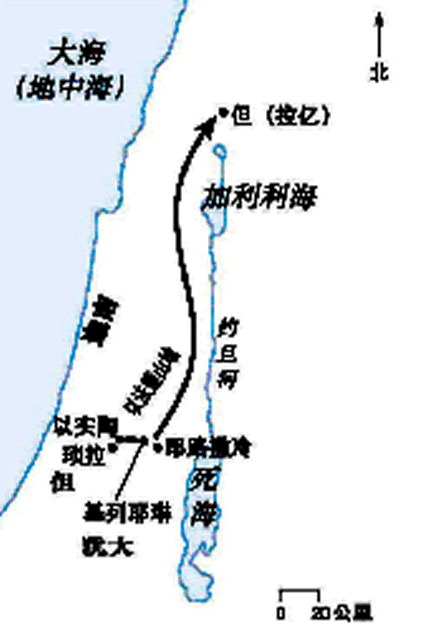
\includegraphics[width=2in]{BLiShiFigs/judge/dan}
	 \caption{但人从琐拉与以实陶定居拉亿}
	 \label{fig:1} 
	 \end{center}
	 \end{wrapfigure}  
他們從那裡往以法蓮山地去，來到米迦的住宅。
從前窺探拉億地的五個人對他們的弟兄說：「這宅子裡有以弗得和家中的神像，並雕刻的像與鑄成的像，你們知道嗎？現在你們要想一想當怎樣行。」 15 五人就進入米迦的住宅，到了那少年利未人的房內問他好。 16 那六百但人各帶兵器，站在門口。 17 窺探地的五個人走進去，將雕刻的像、以弗得、家中的神像並鑄成的像都拿了去；祭司和帶兵器的六百人，一同站在門口。 18 那五個人進入米迦的住宅，拿出雕刻的像、以弗得、家中的神像並鑄成的像，祭司就問他們說：「你們做什麼呢？」 19 他們回答說：「不要作聲，用手摀口，跟我們去吧。我們必以你為父，為祭司。你做一家的祭司好呢，還是做以色列一族一支派的祭司好呢？」 20 祭司心裡喜悅，便拿著以弗得和家中的神像並雕刻的像，進入他們中間。

\subsubsection{但族探地之人鼓励会众前往得地 18:21-26}
他們就轉身離開那裡，妻子、兒女、牲畜、財物都在前頭。 22 離米迦的住宅已遠，米迦的近鄰都聚集來，追趕但人， 23 呼叫但人。但人回頭問米迦說：「你聚集這許多人來做什麼呢？」 24 米迦說：「你們將我所做的神像和祭司都帶了去，我還有所剩的嗎？怎麼還問我說做什麼呢？」 25 但人對米迦說：「你不要使我們聽見你的聲音，恐怕有性暴的人攻擊你，以致你和你的全家盡都喪命。」 26 但人還是走他們的路。米迦見他們的勢力比自己強盛，就轉身回家去了。

\subsubsection{取拉億更名為但 18:27-31}
但人將米迦所做的神像和他的祭司都帶到拉億，見安居無慮的民，就用刀殺了那民，又放火燒了那城。 28 並無人搭救，因為離西頓遠，他們又與別人沒有來往；城在平原，那平原靠近伯利合。但人又在那裡修城居住， 29 照著他們始祖以色列之子但的名字，給那城起名叫但，原先那城名叫拉億。 30 但人就為自己設立那雕刻的像。摩西的孫子、革舜的兒子約拿單和他的子孫做但支派的祭司，直到那地遭擄掠的日子。 31 神的殿在示羅多少日子，但人為自己設立米迦所雕刻的像也在但多少日子。


    
\subsection{利未人和他的妾 19-21}
\subsubsection{利未人至伯利恆迎其行淫離的妾 19:1-9}
當以色列中沒有王的時候，有住以法蓮山地那邊的一個利未人，娶了一個猶大伯利恆的女子為妾。妾行淫離開丈夫，回猶大伯利恆，到了父家，在那裡住了四個月。她丈夫起來，帶著一個僕人、兩匹驢去見她，用好話勸她回來。女子就引丈夫進入父家。她父見了那人，便歡歡喜喜地迎接。那人的岳父，就是女子的父親，將那人留下住了三天。於是二人一同吃喝，住宿。到第四天，利未人清早起來要走，女子的父親對女婿說：「請你吃點飯，加添心力，然後可以行路。」於是二人坐下一同吃喝。女子的父親對那人說：「請你再住一夜，暢快你的心。」那人起來要走，他岳父強留他，他又住了一宿。到第五天，他清早起來要走，女子的父親說：「請你吃點飯，加添心力，等到日頭偏西再走。」於是二人一同吃飯。那人同他的妾和僕人起來要走，他岳父，就是女子的父親，對他說：「看哪，日頭偏西了，請你再住一夜。天快晚了，可以在這裡住宿，暢快你的心，明天早早起行回家去。」

\subsubsection{利未人至基比亞住宿 19:10-21}
那人不願再住一夜，就備上那兩匹驢，帶著妾起身走了，來到耶布斯的對面，耶布斯就是耶路撒冷。 11 臨近耶布斯的時候，日頭快要落了，僕人對主人說：「我們不如進這耶布斯人的城裡住宿。」 12 主人回答說：「我們不可進不是以色列人住的外邦城，不如過到基比亞去。」 13 又對僕人說：「我們可以到一個地方，或住在基比亞，或住在拉瑪。」 14 他們就往前走。將到便雅憫的基比亞，日頭已經落了。 15 他們進入基比亞要在那裡住宿，就坐在城裡的街上，因為無人接他們進家住宿。

晚上，有一個老年人從田間做工回來。他原是以法蓮山地的人，住在基比亞，那地方的人卻是便雅憫人。老年人舉目看見客人坐在城裡的街上，就問他說：「你從哪裡來，要往哪裡去？」他回答說：「我們從猶大伯利恆來，要往以法蓮山地那邊去。我原是那裡的人，到過猶大伯利恆，現在我往耶和華的殿去，在這裡無人接我進他的家。其實我有糧草可以餵驢，我與我的妾並我的僕人有餅有酒，並不缺少什麼。」老年人說：「願你平安！你所需用的我都給你，只是不可在街上過夜。」於是領他們到家裡，餵上驢，他們就洗腳吃喝。

\subsubsection{基比亞匪類之惡行 19:22-28}
\begin{table}[H]
\centering
\begin{tabular}{p{6.5cm}|p{5.cm}|p{5.5cm}}\hline
房主&城中的匪徒&利未人和妾\\\hline
他們心裡正歡暢的時候，
&城中的匪徒圍住房子，連連叩門，對房主老人說：「你把那進你家的人帶出來，我們要與他交合。」&\\\hline
那房主出來對他們說：「弟兄們哪，不要這樣作惡！這人既然進了我的家，你們就不要行這醜事。我有個女兒，還是處女，並有這人的妾，我將她們領出來任憑你們玷辱她們，只是向這人不可行這樣的醜事。」&那些人卻不聽從他的話。&那人就把他的妾拉出去交給他們，\\\hline
&他們便與她交合，終夜凌辱她，直到天色快亮才放她去。 &天快亮的時候，婦人回到她主人住宿的房門前，就仆倒在地，直到天亮。\\\hline
\end{tabular}
\caption{基比亞匪類之惡行 }
\end{table}  

\subsubsection{利未人将惡行通报以色列 19:22-29}
\begin{table}[H]
\centering
\begin{tabular}{p{3.6cm}|p{4.5cm}|p{8.5cm}}\hline
房主&城中的匪徒&利未人和妾\\\hline
早晨她的主人起來，開了房門，出去要行路，
&不料那婦人仆倒在房門前，兩手搭在門檻上。&\\\hline
就對婦人說：「起來，我們走吧！」&婦人卻不回答。那人便將她馱在驢上起身回本處去了。&\\\hline
到了家裡用刀將妾的屍身切成十二塊，使人拿著傳送以色列的四境。& &凡看見的人都說“從以色列人出埃及地直到今日，這樣的事沒有行過也沒有見過！現在應當思想大家商議當怎樣辦理。”\\\hline
\end{tabular}
\caption{利未人将惡行通报以色列}
\end{table}  



\subsubsection{民眾聚集在米斯巴 20:1-7}
\begin{table}[H]
\centering
\begin{tabular}{p{8.6cm}|p{8.5cm}}\hline
以色列民&利未人\\\hline
於是以色列從但到別是巴，以及住基列地的眾人都出來，如同一人，聚集在米斯巴耶和華面前。以色列民的首領，就是各支派的軍長，都站在神百姓的會中，拿刀的步兵共有四十萬。&\multirow{3}{8.5cm}{那利未人，就是被害之婦人的丈夫，回答說：「我和我的妾到了便雅憫的基比亞住宿。基比亞人夜間起來，圍了我住的房子，想要殺我，又將我的妾強姦致死。我就把我妾的屍身切成塊子，使人拿著傳送以色列得為業的全地，因為基比亞人在以色列中行了凶淫醜惡的事。你們以色列人都當籌劃商議。」}\\\cline{1-1}
以色列人上到米斯巴，便雅憫人都聽見了。&\\\cline{1-1}
以色列人說：「請你將這件惡事的情由對我們說明。」&\\\hline
\end{tabular}
\caption{民眾聚集在米斯巴}
\end{table}  


\subsubsection{民眾集議攻討基比亞 20:8-11}
眾民都起來如同一人，說：「我們連一人都不回自己帳篷、自己房屋去。我們向基比亞人必這樣行，照所掣的籤去攻擊他們。我們要在以色列各支派中，一百人挑取十人，一千人挑取百人，一萬人挑取千人，為民運糧，等大眾到了便雅憫的基比亞，就照基比亞人在以色列中所行的醜事征伐他們。」 於是以色列眾人彼此聯合如同一人，聚集攻擊那城。

\subsubsection{便雅憫支派拒交基比亞匪徒 20:12-16}
\begin{table}[H]
\centering
\begin{tabular}{p{6.6cm}|p{10.95cm}}\hline
以色列眾支派&便雅憫\\\hline
以色列眾支派打發人去，問便雅憫支派的各家說：「你們中間怎麼做了這樣的惡事呢？現在你們要將基比亞的那些匪徒交出來，我們好治死他們，從以色列中除掉這惡。」
&便雅憫人卻不肯聽從他們弟兄以色列人的話。便雅憫人從他們的各城裡出來，聚集到了基比亞，要與以色列人打仗。那時便雅憫人從各城裡點出拿刀的，共有二萬六千，另外還有基比亞人點出七百精兵。在眾軍之中有揀選的七百精兵，都是左手便利的，能用機弦甩石打人，毫髮不差。\\\hline
\end{tabular}
\caption{便雅憫支派拒交基比亞匪徒}
\end{table}  


\subsubsection{以色列人初次败于便雅憫 20:17-21}
\begin{table}[H]
\centering
\begin{tabular}{p{8.6cm}|p{2cm}|p{5.5cm}}\hline
以色列眾支派&耶和華&便雅憫\\\hline
便雅憫人之外，點出以色列人拿刀的共有四十萬，都是戰士。以色列人就起來，到伯特利去求問神說：「我們中間誰當首先上去與便雅憫人爭戰呢？」
&耶和華說：「猶大當先上去。」&\\\hline
以色列人早晨起來，對著基比亞安營。以色列人出來，要與便雅憫人打仗，就在基比亞前擺陣。 &&便雅憫人就從基比亞出來，當日殺死以色列人二萬二千。\\\hline
\end{tabular}
\caption{以色列人初次败于便雅憫}
\end{table}  


\subsubsection{以色列人二次败于便雅憫 20:22-25}
\begin{table}[H]
\centering
\begin{tabular}{p{9.6cm}|p{2.5cm}|p{5.cm}}\hline
以色列眾支派&耶和華&便雅憫\\\hline
以色列人彼此奮勇，仍在頭一日擺陣的地方又擺陣。 未擺陣之先，以色列人上去，在耶和華面前哭號，直到晚上，求問耶和華說：「我們再去與我們弟兄便雅憫人打仗可以不可以？」
&耶和華說：「可以上去攻擊他們。」&\\\hline
第二日，以色列人就上前攻擊便雅憫人。&&便雅憫人也在這日從基比亞出來，與以色列人接戰，又殺死他們一萬八千，都是拿刀的。\\\hline
\end{tabular}
\caption{以色列人二次败于便雅憫 }
\end{table}  


\subsubsection{神应许第三次攻討得胜 20:26-28}
\begin{table}[H]
\centering
\begin{tabular}{p{9.6cm}|p{7.5cm}}\hline
以色列眾支派&耶和華\\\hline
以色列眾人就上到伯特利，坐在耶和華面前哭號，當日禁食直到晚上；又在耶和華面前獻燔祭和平安祭。
&那時神的約櫃在那裡，亞倫的孫子、以利亞撒的兒子非尼哈侍立在約櫃前。\\\hline
以色列人問耶和華說：「我們當再出去與我們弟兄便雅憫人打仗呢，還是罷兵呢？」&耶和華說：「你們當上去，因為明日我必將他們交在你們手中。」\\\hline
\end{tabular}
\caption{神应许第三次攻討得胜}
\end{table}  


\subsubsection{便雅憫人敗 20:29-46}
以色列人在基比亞的四圍設下伏兵。 30 第三日，以色列人又上去攻擊便雅憫人，在基比亞前擺陣，與前兩次一樣。 31 便雅憫人也出來迎敵，就被引誘離城。在田間兩條路上，一通伯特利，一通基比亞，像前兩次，動手殺死以色列人約有三十個。 32 便雅憫人說：「他們仍舊敗在我們面前。」但以色列人說：「我們不如逃跑，引誘他們離開城到路上來。」 33 以色列眾人都起來，在巴力他瑪擺陣，以色列的伏兵從馬利迦巴埋伏的地方衝上前去。 34 有以色列人中的一萬精兵，來到基比亞前接戰，勢派甚是凶猛，便雅憫人卻不知道災禍臨近了。 35 耶和華使以色列人殺敗便雅憫人，那日以色列人殺死便雅憫人二萬五千一百，都是拿刀的。

於是便雅憫人知道自己敗了。先是以色列人因為靠著在基比亞前所設的伏兵，就在便雅憫人面前詐敗。 37 伏兵急忙闖進基比亞，用刀殺死全城的人。 38 以色列人預先同伏兵約定在城內放火，以煙氣上騰為號。 39 以色列人臨退陣的時候，便雅憫人動手殺死以色列人，約有三十個，就說：「他們仍像前次被我們殺敗了。」 40 當煙氣如柱從城中上騰的時候，便雅憫人回頭觀看，見全城的煙氣沖天。 41 以色列人又轉身回來，便雅憫人就甚驚惶，因為看見災禍臨到自己了。 42 他們在以色列人面前轉身往曠野逃跑，以色列人在後面追殺，那從各城裡出來的也都夾攻殺滅他們。 43 以色列人圍繞便雅憫人，追趕他們，在他們歇腳之處，對著日出之地的基比亞踐踏他們。 44 便雅憫人死了的有一萬八千，都是勇士。 45 其餘的人轉身向曠野逃跑，往臨門磐去。以色列人在道路上殺了他們五千人，如拾取遺穗一樣，追到基頓又殺了他們二千人。 46 那日便雅憫死了的共有二萬五千人，都是拿刀的勇士。 

\subsubsection{便雅憫人只剩600男人躲在臨門磐 20:47-48}
只剩下六百人，轉身向曠野逃跑，到了臨門磐，就在那裡住了四個月。以色列人又轉到便雅憫地，將各城的人和牲畜並一切所遇見的，都用刀殺盡，又放火燒了一切城邑。

\subsubsection{商议給便雅憫支派娶妻 21:1-7}
以色列人在米斯巴曾起誓說：「我們都不將女兒給便雅憫人為妻。」以色列人來到伯特利，坐在神面前直到晚上，放聲痛哭，說：「耶和華以色列的神啊，為何以色列中有這樣缺了一支派的事呢？」次日清早，百姓起來，在那裡築了一座壇，獻燔祭和平安祭。以色列人彼此問說：「以色列各支派中，誰沒有同會眾上到耶和華面前來呢？」先是以色列人起過大誓說，凡不上米斯巴到耶和華面前來的，必將他治死。以色列人為他們的弟兄便雅憫後悔，說：「如今以色列中絕了一個支派了！我們既在耶和華面前起誓說，必不將我們的女兒給便雅憫人為妻，現在我們當怎樣辦理，使他們剩下的人有妻呢？」
 
\subsubsection{搶四百個處女給便雅憫為妻 21:8-15}
又彼此問說：「以色列支派中誰沒有上米斯巴到耶和華面前來呢？」他們就查出基列雅比沒有一人進營到會眾那裡，因為百姓被數的時候，沒有一個基列雅比人在那裡。會眾就打發一萬二千大勇士，吩咐他們說：「你們去用刀將基列雅比人連婦女帶孩子都擊殺了。所當行的就是這樣，要將一切男子和已嫁的女子盡行殺戮。」他們在基列雅比人中，遇見了四百個未嫁的處女，就帶到迦南地的示羅營裡。全會眾打發人到臨門磐的便雅憫人那裡，向他們說和睦的話。當時便雅憫人回來了，以色列人就把所存活基列雅比的女子給他們為妻，還是不夠。百姓為便雅憫人後悔，因為耶和華使以色列人缺了一個支派 （使以色列中有了破口）。

\subsubsection{搶示羅處女給便雅憫為妻 21:16-25}
\begin{table}[H]
\centering
\begin{tabular}{p{13.cm}|p{4cm}}\hline
以色列眾支派&耶和華\\\hline
會中的長老說：「便雅憫中的女子既然除滅了，我們當怎樣辦理，使那餘剩的人有妻呢？」又說：「便雅憫逃脫的人當有地業，免得以色列中塗抹了一個支派。只是我們不能將自己的女兒給他們為妻，因為以色列人曾起誓說，有將女兒給便雅憫人為妻的，必受咒詛。」他們又說：「在利波拿以南，伯特利以北，在示劍大路以東的示羅，年年有耶和華的節期。」就吩咐便雅憫人說：「你們去，在葡萄園中埋伏。若看見示羅的女子出來跳舞，就從葡萄園出來，在示羅的女子中各搶一個為妻，回便雅憫地去。他們的父親或是弟兄若來與我們爭競，我們就說：『求你們看我們的情面，施恩給這些人，因我們在爭戰的時候沒有給他們留下女子為妻。這也不是你們將女子給他們的；若是你們給的，就算有罪。』」
&於是便雅憫人照樣而行，按著他們的數目從跳舞的女子中搶去為妻，就回自己的地業去，又重修城邑居住。當時以色列人離開那裡，各歸本支派、本宗族、本地業去了。
那時以色列中沒有王，各人任意而行。\\\hline
\end{tabular}
\caption{神应许第三次攻討得胜}
\end{table}  




\chapter{路得記}
\section{以利米勒攜妻及子居摩押地 1:1-18}
\subsection{以利米勒遷居摩押，留下三个寡妇 1:1-5}
\begin{figure}[!htb]  
	 \begin{center}
	 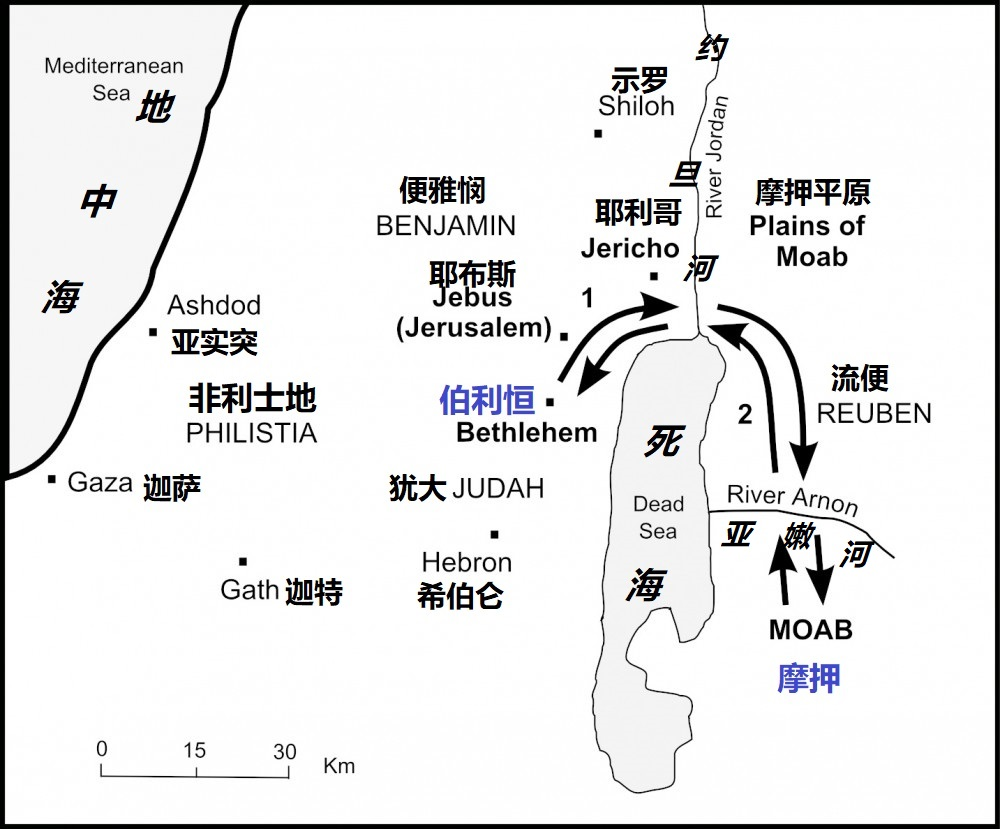
\includegraphics[width=7in]{BLiShiFigs/judge/ruth}
	 \caption{以利米勒遷居摩押}
%	 \label{fig:1} 
	 \end{center}
	 \end{figure}
\begin{table}[H]
\centering
\begin{tabular}{p{8.8cm}|p{7.5cm}}\hline
以利米勒遷居摩押&拿俄米丈夫儿子猝\\\hline
當士師秉政的時候，國中遭遇饑荒。在猶大伯利恆有一個人帶著妻子和兩個兒子，往摩押地去寄居。這人名叫以利米勒，他的妻名叫拿俄米，他兩個兒子，一個名叫瑪倫，一個名叫基連，都是猶大伯利恆的以法他人。他們到了摩押地，就住在那裡。
&後來拿俄米的丈夫以利米勒死了，剩下婦人和她兩個兒子。這兩個兒子娶了摩押女子為妻，一個名叫俄珥巴，一個名叫路得，在那裡住了約有十年。瑪倫和基連二人也死了，剩下拿俄米，沒有丈夫，也沒有兒子。\\\hline
\end{tabular}
\caption{兒婦俄珥巴與婆婆親嘴而別}
\end{table} 


%\subsection{拿俄米丈夫儿子猝 1:3-5}


%\subsection{拿俄米要回猶大地 1:6-7}


\subsection{兒婦俄珥巴與婆婆親嘴而別 1:6-14}
\begin{table}[H]
\centering
\begin{tabular}{p{12.8cm}|p{4.5cm}}\hline
拿俄米&兩個兒婦\\\hline
她就與兩個兒婦起身，要從摩押地歸回，因為她在摩押地聽見耶和華眷顧自己的百姓，賜糧食於他們。於是她和兩個兒婦起行離開所住的地方，要回猶大地去。拿俄米對兩個兒婦說：「你們各人回娘家去吧！願耶和華恩待你們，像你們恩待已死的人與我一樣。願耶和華使你們各在新夫家中得平安。」於是拿俄米與她們親嘴，
&她們就放聲而哭說：「不然，我們必與你一同回你本國去。」 \\\hline
拿俄米說：「我女兒們哪，回去吧！為何要跟我去呢？我還能生子做你們的丈夫嗎？我女兒們哪，回去吧！我年紀老邁，不能再有丈夫。即或說我還有指望，今夜有丈夫可以生子，你們豈能等著他們長大呢？你們豈能等著他們不嫁別人呢？我女兒們哪，不要這樣！我為你們的緣故，甚是愁苦，因為耶和華伸手攻擊我。」&兩個兒婦又放聲而哭，俄珥巴與婆婆親嘴而別，\\\hline
\end{tabular}
\caption{兒婦俄珥巴與婆婆親嘴而別}
\end{table} 


\subsection{路得定意跟隨拿俄米回伯利恆 1:15-18}
\begin{table}[H]
\centering
\begin{tabular}{p{12.cm}|p{5cm}}\hline
路得&拿俄米\\\hline
只是路得捨不得拿俄米。
&拿俄米說：「看哪，你嫂子已經回她本國和她所拜的神那裡去了，你也跟著你嫂子回去吧！」 \\\hline
路得說：「不要催我回去不跟隨你！你往哪裡去我也往哪裡去；你在哪裡住宿我也在哪裡住宿。你的國就是我的國，你的神就是我的神。你在哪裡死，我也在哪裡死也葬在那裡。除非死能使你我相離，不然願耶和華重重地降罰於我！」 &拿俄米見路得定意要跟隨自己去，就不再勸她了。\\\hline
\end{tabular}
\caption{路得定意跟隨拿俄米回伯利恆}
\end{table} 



\section{拿俄米和路得回到伯利恆 1:19-2:23}
\subsection{拿俄米和路得回到伯利恆 1:19-22}
於是二人同行，來到伯利恆。她們到了伯利恆，合城的人就都驚訝。婦女們說：「這是拿俄米嗎？」 20 拿俄米對她們說：「不要叫我拿俄米（甜），要叫我瑪拉（苦），因為全能者使我受了大苦。 21 我滿滿地出去，耶和華使我空空地回來。耶和華降禍於我，全能者使我受苦。既是這樣，你們為何還叫我拿俄米呢？」拿俄米和她兒婦摩押女子路得從摩押地回來到伯利恆，正是動手割大麥的時候。

\subsection{路得在波阿斯田間拾取麥穗 2:1-3}
\begin{table}[H]
\centering
\begin{tabular}{p{5.5cm}|p{8.5cm}|p{3cm}}\hline
波阿斯&路得&拿俄米\\\hline
拿俄米的丈夫以利米勒的親族中，有一個人名叫波阿斯，是個大財主。 
&摩押女子路得對拿俄米說：「容我往田間去，我蒙誰的恩，就在誰的身後拾取麥穗。」 &拿俄米說：「女兒啊，你只管去。」\\\hline
&路得就去了，來到田間，在收割的人身後拾取麥穗。她恰巧到了以利米勒本族的人波阿斯那塊田裡。&\\\hline
\end{tabular}
\caption{路得在波阿斯田間拾取麥穗 }
\end{table} 


\subsection{波阿斯遇到路得 2:4-7}
\begin{table}[H]
\centering
\begin{tabular}{p{5.cm}|p{5.5cm}|p{6.5cm}}\hline
波阿斯&收割的人&路得\\\hline
波阿斯正從伯利恆來，對收割的人說：「願耶和華與你們同在！」
&他們回答說：「願耶和華賜福於你！」 & \\\hline
波阿斯問監管收割的僕人說：「那是誰家的女子？」 &監管收割的僕人回答說：「是那摩押女子，跟隨拿俄米從摩押地回來的。&
她說：『請你容我跟著收割的人，拾取打捆剩下的麥穗。』她從早晨直到如今，除了在屋子裡坐一會兒，常在這裡。」\\\hline
\end{tabular}
\caption{波阿斯遇到路得}
\end{table} 


\subsection{波阿斯厚遇路得 2:8-18}
\begin{table}[H]
\centering
\begin{tabular}{p{9.cm}|p{8.cm}}\hline
波阿斯&路得\\\hline
波阿斯對路得說：「女兒啊，聽我說，不要往別人田裡拾取麥穗，也不要離開這裡，要常與我使女們在一處。我的僕人在哪塊田收割，你就跟著他們去。我已經吩咐僕人不可欺負你。你若渴了，就可以到器皿那裡喝僕人打來的水。」
&路得就俯伏在地叩拜，對他說：「我既是外邦人，怎麼蒙你的恩，這樣顧恤我呢？」 \\\hline
波阿斯回答說：「自從你丈夫死後，凡你向婆婆所行的，並你離開父母和本地到素不認識的民中，這些事，人全都告訴我了。願耶和華照你所行的賞賜你。你來投靠耶和華以色列神的翅膀下，願你滿得他的賞賜。」 &路得說：「我主啊，願在你眼前蒙恩。我雖然不及你的一個使女，你還用慈愛的話安慰我的心。」
\\\hline
到了吃飯的時候，波阿斯對路得說：「你到這裡來吃餅，將餅蘸在醋裡。」&
路得就在收割的人旁邊坐下。他們把烘了的穗子遞給她，她吃飽了，還有餘剩的。她起來又拾取麥穗。\\\hline
波阿斯吩咐僕人說：「她就是在捆中拾取麥穗，也可以容她，不可羞辱她；並要從捆裡抽出些來，留在地下任她拾取，不可叱嚇她。」&這樣，路得在田間拾取麥穗，直到晚上。將所拾取的打了，約有一伊法大麥。她就把所拾取的帶進城去給婆婆看，又把她吃飽了所剩的給了婆婆。\\\hline
\end{tabular}
\caption{波阿斯遇到路得}
\end{table} 

\subsection{拿俄米嘱咐路得只在波阿斯田間拾取麥穗 2:19-23}
\begin{table}[H]
\centering
\begin{tabular}{p{8.cm}|p{8.5cm}}\hline
婆婆&路得\\\hline
婆婆問她說：「你今日在哪裡拾取麥穗，在哪裡做工呢？願那顧恤你的得福！」
&路得就告訴婆婆說：「我今日在一個名叫波阿斯的人那裡做工。」  \\\hline
拿俄米對兒婦說：「願那人蒙耶和華賜福！因為他不斷地恩待活人死人。」拿俄米又說：「那是我們本族的人，是一個至近的親屬。」&摩押女子路得說：「他對我說：『你要緊隨我的僕人拾取麥穗，直等他們收完了我的莊稼。』」 \\\hline
拿俄米對兒婦路得說：「女兒啊，你跟著他的使女出去，不叫人遇見你在別人田間，這才為好。」&
於是路得與波阿斯的使女常在一處拾取麥穗，直到收完了大麥和小麥。路得仍與婆婆同住。\\\hline
\end{tabular}
\caption{拿俄米嘱咐路得只在波阿斯田間拾取麥穗}
\end{table} 


 

\section{拿俄米求波阿斯赎地 3:1-4:6}
\subsection{拿俄米給路得出主意 3:1-5 }
\begin{table}[H]
\centering
\begin{tabular}{p{15.5cm}|p{1.7cm}}\hline
婆婆拿俄米&路得\\\hline
路得的婆婆拿俄米對她說：「女兒啊，我不當為你找個安身之處，使你享福嗎？ 你與波阿斯的使女常在一處，波阿斯不是我們的親族嗎？他今夜在場上簸大麥，你要沐浴抹膏，換上衣服，下到場上，卻不要使那人認出你來。你等他吃喝完了，到他睡的時候，你看準他睡的地方，就進去掀開他腳上的被，躺臥在那裡。他必告訴你所當做的事。」 &路得說：「凡你所吩咐的，我必遵行。」\\\hline
\end{tabular}
\caption{拿俄米給路得出主意}
\end{table} 

\subsection{路得求波阿斯遮蓋 3:6-15}
\begin{table}[H]
\centering
\begin{tabular}{p{6.7cm}|p{10.3cm}}\hline
路得&波阿斯\\\hline
路得就下到場上，照她婆婆所吩咐她的而行。&波阿斯吃喝完了，心裡歡暢，就去睡在麥堆旁邊。\\\hline
路得便悄悄地來掀開他腳上的被，躺臥在那裡。&到了夜半，那人忽然驚醒，翻過身來，不料有女子躺在他的腳下。他就說：「你是誰？」\\\hline
回答說：「我是你的婢女路得。求你用你的衣襟遮蓋我，因為你是我一個至近的親屬。」 &波阿斯說：「女兒啊，願你蒙耶和華賜福！你末後的恩比先前更大，因為少年人無論貧富，你都沒有跟從。女兒啊，現在不要懼怕，凡你所說的，我必照著行。我本城的人都知道你是個賢德的女子。我實在是你一個至近的親屬，只是還有一個人比我更近。你今夜在這裡住宿，明早他若肯為你盡親屬的本分，就由他吧。倘若不肯，我指著永生的耶和華起誓：我必為你盡了本分！你只管躺到天亮。」\\\hline
路得便在他腳下躺到天快亮，人彼此不能辨認的時候就起來了。&波阿斯說：「不可使人知道有女子到場上來。」又對路得說：「打開你所披的外衣。」\\\hline
她打開了，&波阿斯就撮了六簸箕大麥，幫她扛在肩上，\\\hline
她便進城去了。&\\\hline
\end{tabular}
\caption{路得求波阿斯遮蓋}
\end{table} 

\subsection{拿俄米安慰路得 3:16-18}
\begin{table}[H]
\centering
\begin{tabular}{p{8.5cm}|p{8.7cm}}\hline
婆婆拿俄米&路得\\\hline
路得回到婆婆那裡，&婆婆說：「女兒啊，怎麼樣了？」\\\hline
路得就將那人向她所行的述說了一遍。又說：「那人給了我六簸箕大麥，對我說：『你不可空手回去見你的婆婆。』」 &婆婆說：「女兒啊，你只管安坐等候，看這事怎樣成就，因為那人今日不辦成這事必不休息。」\\\hline
 \end{tabular}
\caption{拿俄米安慰路得}
\end{table} 


\subsection{波阿斯与那人谈贖以利米勒之產 4:1-6}
\begin{table}[H]
\centering
\begin{tabular}{p{10.5cm}|p{6.7cm}}\hline
波阿斯&那人/眾民和長老\\\hline
波阿斯到了城門，坐在那裡，&恰巧波阿斯所說的那至近的親屬經過。\\\hline
波阿斯對長老和眾民說"你們今日做見證:凡屬以利米勒和基連、瑪倫的，我波阿斯說：「某人哪，你來坐在這裡。」&他就來坐下。\\\hline
波阿斯又從本城的長老中揀選了十人，對他們說：「請你們坐在這裡。」&他們就都坐下。 \\\hline
波阿斯對那至近的親屬說：「從摩押地回來的拿俄米，現在要賣我們族兄以利米勒的那塊地。我想當贖那塊地的是你，其次是我，以外再沒有別人了。你可以在這裡的人面前和我本國的長老面前說明，你若肯贖就贖，若不肯贖就告訴我。」&那人回答說：「我肯贖。」 \\\hline
波阿斯說：「你從拿俄米手中買這地的時候，也當娶（買）死人的妻摩押女子路得，使死人在產業上存留他的名。」 &那人說“這樣我就不能贖了恐怕於我的產業有礙。你可以贖我所當贖的我不能贖了”\\\hline
\end{tabular}
\caption{波阿斯得到买赎地的权力}
\end{table} 


\section{波阿斯迎娶路得 4:7-22}
\subsection{波阿斯得到买赎地的权力 4:7-12}
\begin{table}[H]
\centering
\begin{tabular}{p{2.5cm}|p{1.7cm}|p{5.8cm}|p{6.1cm}}\hline
以色列&那人&波阿斯&眾民和長老\\\hline
從前在以色列中要定奪什麼事,或贖回或交易,這人就脫鞋給那人。以色列人都以此為證據。
&那人對波阿斯說"你自己買吧。"於是將鞋脫下來了。
&波阿斯對長老和眾民說"你們今日做見證:凡屬以利米勒和基連、瑪倫的，我都從拿俄米手中置買了;又娶了瑪倫的妻摩押女子路得為妻,好在死人的產業上存留他的名,免得他的名在本族本鄉滅沒。你們今日可以做見證"
&在城門坐著的眾民和長老都說"我們做見證。願耶和華使進你家的這女子像建立以色列家的拉結、利亞二人一樣！又願你在以法他得亨通,在伯利恆得名聲！願耶和華從這少年女子賜你後裔,使你的家像她瑪從猶大所生法勒斯的家一般!"\\\hline
\end{tabular}
\caption{波阿斯得到买赎地的权力}
\end{table} 



\subsection{波阿斯的後代 4:13-22 }
於是，波阿斯娶了路得為妻，與她同房。耶和華使她懷孕生了一個兒子。婦人們對拿俄米說：「耶和華是應當稱頌的！因為今日沒有撇下你，使你無至近的親屬。願這孩子在以色列中得名聲！他必提起你的精神，奉養你的老，因為是愛慕你的那兒婦所生的。有這兒婦比有七個兒子還好。」拿俄米就把孩子抱在懷中，做他的養母。鄰舍的婦人說：「拿俄米得孩子了。」就給孩子起名叫俄備得。這俄備得是耶西的父，耶西是大衛的父。

法勒斯的後代記在下面：法勒斯生希斯崙，希斯崙生蘭，蘭生亞米拿達，亞米拿達生拿順，拿順生撒門，撒門生波阿斯，波阿斯生俄備得， 俄備得生耶西，耶西生大衛。

\begin{forest}
  for tree={
    child anchor=west,
    parent anchor=east,
    grow=east,
    draw,
    anchor=west,
    edge path={
      \noexpand\path[\forestoption{edge}]
        (.child anchor) -| +(-5pt,0) -- +(-5pt,0) |-
        (!u.parent anchor)\forestoption{edge label};
    },
  }
  [法勒斯[希斯崙[蘭[亞米拿達[拿順[撒門[喇合（撒門妻子，生波阿斯）][\textbf{波阿斯}[路得（波阿斯妻子，生俄備得）][俄備得[耶西[大衛]]]]]]]]]]
  ]
\end{forest}



